\documentclass[12pt,leqno]{article}
%\documentclass[a4paper,12pt,twoside]{article}
%\documentclass[14pt,a4paper]{scrbook}

%\usepackage{float}
%\usepackage{listings}
%\usepackage{xkeyval}
%\usepackage{eucal}
%\usepackage{mathrsfs}
%\usepackage{theorem}
%\usepackage{pifont}
% \usepackage{bibtopic,wrapfig}
%\usepackage{bbding}
%\usepackage{fancyhdr}
%\usepackage{verbatim}
%\usepackage{bidi}




%\rhead{\thepage}
%\lfoot{\small \copyright\;\;\; שירה בר-דב, אורט בראודה}
%\rfoot{\thepage}
%\cfoot{}
%\renewcommand{\headrulewidth}{0.4pt}
%\renewcommand{\footrulewidth}{0.4pt}
%\DeclareGraphicsExtensions{.pdf,.png,.jpg}
%\let\arref\ref
%\renewcommand{\ref}[1]{\I{\arref{#1}}}




%\rhead{\thepage}
%\lfoot{\small \copyright\;\;\; שירה בר-דב, אורט בראודה}
%\rfoot{\thepage}
%\cfoot{}
%\renewcommand{\headrulewidth}{0.4pt}
%\renewcommand{\footrulewidth}{0.4pt}
%\DeclareGraphicsExtensions{.pdf,.png,.jpg}
%\let\arref\ref
%\renewcommand{\ref}[1]{\I{\arref{#1}}}

% \setlength{\parskip}{4pt plus 2pt} \setlength{\parindent}{0pt}
% \setlength{\oddsidemargin}{0pt} \setlength{\evensidemargin}{0pt}

%\numberwithin{equation}{section}

%\documentclass{amsart}
%%\usepackage[active]{srcltx} % SRC Specials for DVI Searching
%\usepackage {epsfig}
%% THEOREM Environments ---------------------------------------------------
% \newtheorem{thm}{Theorem}
% \newtheorem{cor}[thm]{Corollary}
% \newtheorem{lemma}[thm]{Lemma}
% \newtheorem{prop}[thm]{Proposition}
% \newtheorem{theorem}[thm]{Theorem}
% \theoremstyle{definition}
% \newtheorem{defn}[thm]{Definition}
% \theoremstyle{remark}
% \newtheorem{rem}[thm]{Remark}
%% MATH -------------------------------------------------------------------
%%%% ----------------------------------------------------------------------
%\setlength{\textheight}{43pc} \setlength{\textwidth}{28pc}
%

%%%%%% Jupyter paereamble
%\pagenumbering{gobble}
\usepackage[breakable]{tcolorbox}
\usepackage{parskip} % Stop auto-indenting (to mimic markdown behaviour)

\usepackage{iftex}
\usepackage{mathpazo}

% Basic figure setup, for now with no caption control since it's done
% automatically by Pandoc (which extracts ![](path) syntax from Markdown).
\usepackage{graphicx}
% Maintain compatibility with old templates. Remove in nbconvert 6.0
\let\Oldincludegraphics\includegraphics
% Ensure that by default, figures have no caption (until we provide a
% proper Figure object with a Caption API and a way to capture that
% in the conversion process - todo).
\usepackage{caption}
%\DeclareCaptionFormat{nocaption}{}
%\captionsetup{format=nocaption,aboveskip=0pt,belowskip=0pt}

\usepackage{float}
\floatplacement{figure}{H} % forces figures to be placed at the correct location
\usepackage{xcolor} % Allow colors to be defined
\usepackage{enumerate} % Needed for markdown enumerations to work
%\usepackage{geometry} % Used to adjust the document margins
% \usepackage{amsmath} % Equations
% \usepackage{amssymb} % Equations
\usepackage{textcomp} % defines textquotesingle
% Hack from http://tex.stackexchange.com/a/47451/13684:
\AtBeginDocument{%
    \def\PYZsq{\textquotesingle}% Upright quotes in Pygmentized code
}
\usepackage{upquote} % Upright quotes for verbatim code
\usepackage{eurosym} % defines \euro
\usepackage[mathletters]{ucs} % Extended unicode (utf-8) support
\usepackage{fancyvrb} % verbatim replacement that allows latex
\usepackage{grffile} % extends the file name processing of package graphics 
                        % to support a larger range
\makeatletter % fix for old versions of grffile with XeLaTeX
\@ifpackagelater{grffile}{2019/11/01}
{
    % Do nothing on new versions
}
{
    \def\Gread@@xetex#1{%
    \IfFileExists{"\Gin@base".bb}%
    {\Gread@eps{\Gin@base.bb}}%
    {\Gread@@xetex@aux#1}%
    }
}
\makeatother
\usepackage[Export]{adjustbox} % Used to constrain images to a maximum size
\adjustboxset{max size={0.9\linewidth}{0.9\paperheight}}

% The hyperref package gives us a pdf with properly built
% internal navigation ('pdf bookmarks' for the table of contents,
% internal cross-reference links, web links for URLs, etc.)
% \usepackage{hyperref}
% The default LaTeX title has an obnoxious amount of whitespace. By default,
% titling removes some of it. It also provides customization options.
\usepackage{titling}
\usepackage{longtable} % long table support required by pandoc >1.10
\usepackage{booktabs}  % table support for pandoc > 1.12.2
\usepackage[inline]{enumitem} % IRkernel/repr support (it uses the enumerate* environment)
\usepackage[normalem]{ulem} % ulem is needed to support strikethroughs (\sout)
                            % normalem makes italics be italics, not underlines
\usepackage{mathrsfs}
    



% User packages
%%%%%%%%%%%%%%%%%%%%%%%%%%%%%%%%
\usepackage{amsmath,amssymb}
\usepackage{amsthm}
\usepackage{import}
%\theoremstyle{plain}
\newtheoremstyle{theoremdd}% name of the style to be used
  {\topsep}% measure of space to leave above the theorem. E.g.: 3pt
  {\topsep}% measure of space to leave below the theorem. E.g.: 3pt
  {\itshape}% name of font to use in the body of the theorem
  {0pt}% measure of space to indent
  {\bfseries}% name of head font
  {:}% punctuation between head and body
  { }% space after theorem head; " " = normal inter word space
  {\thmname{#1}\thmnumber{ #2}\thmnote{ #3}} % Manually specify head
\theoremstyle{theoremdd}
% \usepackage{graphicx}
% \usepackage{pgfplots}
%\usepackage{color} %red, green, blue, yellow, cyan, magenta, black, white
% \definecolor{mygreen}{RGB}{28,172,0} % color values Red, Green, Blue
% \definecolor{mylilas}{RGB}{170,55,241}
% \usepackage{graphicx}
% \usepackage{epstopdf}
% \usepackage{epsfig}
\usepackage[hyperindex,colorlinks]{hyperref}
%\usepackage[colorlinks=true, bookmarks=true]{hyperref}
\usepackage{subcaption}
%\usepackage{mathtools}
%\usepackage{pdfpages}
\linespread{1.4}
\usepackage[lmargin=1in,rmargin=1in,tmargin=1in]{geometry}
\usepackage{xcolor}
\usepackage{fontspec}
\usepackage{polyglossia}
\usepackage{array}
\setdefaultlanguage{hebrew}
\setotherlanguages{english}
\newfontfamily\hebrewfont[Script=Hebrew]{David}
% It's a clear bug in how Polyglossia manages the situation, 
% as it seems not taking into account the current language. 
% A temporary workaround is to say
% This assuming that you don't need Hebrew in the minted environment.
\let\hebrewfonttt\ttfamily
%\usepackage{bidi}

% User defined macros
%%%%%%%%%%%%%%%%%%%%%%%%%%%%%%%%
\newtheorem{definition}{הגדרה}
\newtheorem{theorem}{משפט}
\newtheorem{proposition}{טענה}
\newtheorem{conjecture}{השערה}
\newtheorem{corollary}{מסקנה}
\newtheorem{lemma}{למה}
\newtheorem{example}{דוגמה}
\newtheorem{comm}{הערה}

\newcommand{\sumi}[1]{\sum_{#1=1}^n}
\newcommand{\Zn}{{\mathbb{Z}_2}^n}
\newcommand{\Col}{\mathrm{Col}}
\newcommand{\Nul}{\mathrm{Nul}}
    

    
    % Colors for the hyperref package
    \definecolor{urlcolor}{rgb}{0,.145,.698}
    \definecolor{linkcolor}{rgb}{.71,0.21,0.01}
    \definecolor{citecolor}{rgb}{.12,.54,.11}

    % ANSI colors
    \definecolor{ansi-black}{HTML}{3E424D}
    \definecolor{ansi-black-intense}{HTML}{282C36}
    \definecolor{ansi-red}{HTML}{E75C58}
    \definecolor{ansi-red-intense}{HTML}{B22B31}
    \definecolor{ansi-green}{HTML}{00A250}
    \definecolor{ansi-green-intense}{HTML}{007427}
    \definecolor{ansi-yellow}{HTML}{DDB62B}
    \definecolor{ansi-yellow-intense}{HTML}{B27D12}
    \definecolor{ansi-blue}{HTML}{208FFB}
    \definecolor{ansi-blue-intense}{HTML}{0065CA}
    \definecolor{ansi-magenta}{HTML}{D160C4}
    \definecolor{ansi-magenta-intense}{HTML}{A03196}
    \definecolor{ansi-cyan}{HTML}{60C6C8}
    \definecolor{ansi-cyan-intense}{HTML}{258F8F}
    \definecolor{ansi-white}{HTML}{C5C1B4}
    \definecolor{ansi-white-intense}{HTML}{A1A6B2}
    \definecolor{ansi-default-inverse-fg}{HTML}{FFFFFF}
    \definecolor{ansi-default-inverse-bg}{HTML}{000000}

    % common color for the border for error outputs.
    \definecolor{outerrorbackground}{HTML}{FFDFDF}

    % commands and environments needed by pandoc snippets
    % extracted from the output of `pandoc -s`
    \providecommand{\tightlist}{%
      \setlength{\itemsep}{0pt}\setlength{\parskip}{0pt}}
    \DefineVerbatimEnvironment{Highlighting}{Verbatim}{commandchars=\\\{\}}
    % Add ',fontsize=\small' for more characters per line
    \newenvironment{Shaded}{}{}
    \newcommand{\KeywordTok}[1]{\textcolor[rgb]{0.00,0.44,0.13}{\textbf{{#1}}}}
    \newcommand{\DataTypeTok}[1]{\textcolor[rgb]{0.56,0.13,0.00}{{#1}}}
    \newcommand{\DecValTok}[1]{\textcolor[rgb]{0.25,0.63,0.44}{{#1}}}
    \newcommand{\BaseNTok}[1]{\textcolor[rgb]{0.25,0.63,0.44}{{#1}}}
    \newcommand{\FloatTok}[1]{\textcolor[rgb]{0.25,0.63,0.44}{{#1}}}
    \newcommand{\CharTok}[1]{\textcolor[rgb]{0.25,0.44,0.63}{{#1}}}
    \newcommand{\StringTok}[1]{\textcolor[rgb]{0.25,0.44,0.63}{{#1}}}
    \newcommand{\CommentTok}[1]{\textcolor[rgb]{0.38,0.63,0.69}{\textit{{#1}}}}
    \newcommand{\OtherTok}[1]{\textcolor[rgb]{0.00,0.44,0.13}{{#1}}}
    \newcommand{\AlertTok}[1]{\textcolor[rgb]{1.00,0.00,0.00}{\textbf{{#1}}}}
    \newcommand{\FunctionTok}[1]{\textcolor[rgb]{0.02,0.16,0.49}{{#1}}}
    \newcommand{\RegionMarkerTok}[1]{{#1}}
    \newcommand{\ErrorTok}[1]{\textcolor[rgb]{1.00,0.00,0.00}{\textbf{{#1}}}}
    \newcommand{\NormalTok}[1]{{#1}}
    
    % Additional commands for more recent versions of Pandoc
    \newcommand{\ConstantTok}[1]{\textcolor[rgb]{0.53,0.00,0.00}{{#1}}}
    \newcommand{\SpecialCharTok}[1]{\textcolor[rgb]{0.25,0.44,0.63}{{#1}}}
    \newcommand{\VerbatimStringTok}[1]{\textcolor[rgb]{0.25,0.44,0.63}{{#1}}}
    \newcommand{\SpecialStringTok}[1]{\textcolor[rgb]{0.73,0.40,0.53}{{#1}}}
    \newcommand{\ImportTok}[1]{{#1}}
    \newcommand{\DocumentationTok}[1]{\textcolor[rgb]{0.73,0.13,0.13}{\textit{{#1}}}}
    \newcommand{\AnnotationTok}[1]{\textcolor[rgb]{0.38,0.63,0.69}{\textbf{\textit{{#1}}}}}
    \newcommand{\CommentVarTok}[1]{\textcolor[rgb]{0.38,0.63,0.69}{\textbf{\textit{{#1}}}}}
    \newcommand{\VariableTok}[1]{\textcolor[rgb]{0.10,0.09,0.49}{{#1}}}
    \newcommand{\ControlFlowTok}[1]{\textcolor[rgb]{0.00,0.44,0.13}{\textbf{{#1}}}}
    \newcommand{\OperatorTok}[1]{\textcolor[rgb]{0.40,0.40,0.40}{{#1}}}
    \newcommand{\BuiltInTok}[1]{{#1}}
    \newcommand{\ExtensionTok}[1]{{#1}}
    \newcommand{\PreprocessorTok}[1]{\textcolor[rgb]{0.74,0.48,0.00}{{#1}}}
    \newcommand{\AttributeTok}[1]{\textcolor[rgb]{0.49,0.56,0.16}{{#1}}}
    \newcommand{\InformationTok}[1]{\textcolor[rgb]{0.38,0.63,0.69}{\textbf{\textit{{#1}}}}}
    \newcommand{\WarningTok}[1]{\textcolor[rgb]{0.38,0.63,0.69}{\textbf{\textit{{#1}}}}}
    
    
    % Define a nice break command that doesn't care if a line doesn't already
    % exist.
    \def\br{\hspace*{\fill} \\* }
    % Math Jax compatibility definitions
    \def\gt{>}
    \def\lt{<}
    \let\Oldtex\TeX
    \let\Oldlatex\LaTeX
    \renewcommand{\TeX}{\textrm{\Oldtex}}
    \renewcommand{\LaTeX}{\textrm{\Oldlatex}}
    % Document parameters
    % Document title
    \title{light\_out}
    
    
    
    
    
% Pygments definitions
\makeatletter
\def\PY@reset{\let\PY@it=\relax \let\PY@bf=\relax%
    \let\PY@ul=\relax \let\PY@tc=\relax%
    \let\PY@bc=\relax \let\PY@ff=\relax}
\def\PY@tok#1{\csname PY@tok@#1\endcsname}
\def\PY@toks#1+{\ifx\relax#1\empty\else%
    \PY@tok{#1}\expandafter\PY@toks\fi}
\def\PY@do#1{\PY@bc{\PY@tc{\PY@ul{%
    \PY@it{\PY@bf{\PY@ff{#1}}}}}}}
\def\PY#1#2{\PY@reset\PY@toks#1+\relax+\PY@do{#2}}

\@namedef{PY@tok@w}{\def\PY@tc##1{\textcolor[rgb]{0.73,0.73,0.73}{##1}}}
\@namedef{PY@tok@c}{\let\PY@it=\textit\def\PY@tc##1{\textcolor[rgb]{0.25,0.50,0.50}{##1}}}
\@namedef{PY@tok@cp}{\def\PY@tc##1{\textcolor[rgb]{0.74,0.48,0.00}{##1}}}
\@namedef{PY@tok@k}{\let\PY@bf=\textbf\def\PY@tc##1{\textcolor[rgb]{0.00,0.50,0.00}{##1}}}
\@namedef{PY@tok@kp}{\def\PY@tc##1{\textcolor[rgb]{0.00,0.50,0.00}{##1}}}
\@namedef{PY@tok@kt}{\def\PY@tc##1{\textcolor[rgb]{0.69,0.00,0.25}{##1}}}
\@namedef{PY@tok@o}{\def\PY@tc##1{\textcolor[rgb]{0.40,0.40,0.40}{##1}}}
\@namedef{PY@tok@ow}{\let\PY@bf=\textbf\def\PY@tc##1{\textcolor[rgb]{0.67,0.13,1.00}{##1}}}
\@namedef{PY@tok@nb}{\def\PY@tc##1{\textcolor[rgb]{0.00,0.50,0.00}{##1}}}
\@namedef{PY@tok@nf}{\def\PY@tc##1{\textcolor[rgb]{0.00,0.00,1.00}{##1}}}
\@namedef{PY@tok@nc}{\let\PY@bf=\textbf\def\PY@tc##1{\textcolor[rgb]{0.00,0.00,1.00}{##1}}}
\@namedef{PY@tok@nn}{\let\PY@bf=\textbf\def\PY@tc##1{\textcolor[rgb]{0.00,0.00,1.00}{##1}}}
\@namedef{PY@tok@ne}{\let\PY@bf=\textbf\def\PY@tc##1{\textcolor[rgb]{0.82,0.25,0.23}{##1}}}
\@namedef{PY@tok@nv}{\def\PY@tc##1{\textcolor[rgb]{0.10,0.09,0.49}{##1}}}
\@namedef{PY@tok@no}{\def\PY@tc##1{\textcolor[rgb]{0.53,0.00,0.00}{##1}}}
\@namedef{PY@tok@nl}{\def\PY@tc##1{\textcolor[rgb]{0.63,0.63,0.00}{##1}}}
\@namedef{PY@tok@ni}{\let\PY@bf=\textbf\def\PY@tc##1{\textcolor[rgb]{0.60,0.60,0.60}{##1}}}
\@namedef{PY@tok@na}{\def\PY@tc##1{\textcolor[rgb]{0.49,0.56,0.16}{##1}}}
\@namedef{PY@tok@nt}{\let\PY@bf=\textbf\def\PY@tc##1{\textcolor[rgb]{0.00,0.50,0.00}{##1}}}
\@namedef{PY@tok@nd}{\def\PY@tc##1{\textcolor[rgb]{0.67,0.13,1.00}{##1}}}
\@namedef{PY@tok@s}{\def\PY@tc##1{\textcolor[rgb]{0.73,0.13,0.13}{##1}}}
\@namedef{PY@tok@sd}{\let\PY@it=\textit\def\PY@tc##1{\textcolor[rgb]{0.73,0.13,0.13}{##1}}}
\@namedef{PY@tok@si}{\let\PY@bf=\textbf\def\PY@tc##1{\textcolor[rgb]{0.73,0.40,0.53}{##1}}}
\@namedef{PY@tok@se}{\let\PY@bf=\textbf\def\PY@tc##1{\textcolor[rgb]{0.73,0.40,0.13}{##1}}}
\@namedef{PY@tok@sr}{\def\PY@tc##1{\textcolor[rgb]{0.73,0.40,0.53}{##1}}}
\@namedef{PY@tok@ss}{\def\PY@tc##1{\textcolor[rgb]{0.10,0.09,0.49}{##1}}}
\@namedef{PY@tok@sx}{\def\PY@tc##1{\textcolor[rgb]{0.00,0.50,0.00}{##1}}}
\@namedef{PY@tok@m}{\def\PY@tc##1{\textcolor[rgb]{0.40,0.40,0.40}{##1}}}
\@namedef{PY@tok@gh}{\let\PY@bf=\textbf\def\PY@tc##1{\textcolor[rgb]{0.00,0.00,0.50}{##1}}}
\@namedef{PY@tok@gu}{\let\PY@bf=\textbf\def\PY@tc##1{\textcolor[rgb]{0.50,0.00,0.50}{##1}}}
\@namedef{PY@tok@gd}{\def\PY@tc##1{\textcolor[rgb]{0.63,0.00,0.00}{##1}}}
\@namedef{PY@tok@gi}{\def\PY@tc##1{\textcolor[rgb]{0.00,0.63,0.00}{##1}}}
\@namedef{PY@tok@gr}{\def\PY@tc##1{\textcolor[rgb]{1.00,0.00,0.00}{##1}}}
\@namedef{PY@tok@ge}{\let\PY@it=\textit}
\@namedef{PY@tok@gs}{\let\PY@bf=\textbf}
\@namedef{PY@tok@gp}{\let\PY@bf=\textbf\def\PY@tc##1{\textcolor[rgb]{0.00,0.00,0.50}{##1}}}
\@namedef{PY@tok@go}{\def\PY@tc##1{\textcolor[rgb]{0.53,0.53,0.53}{##1}}}
\@namedef{PY@tok@gt}{\def\PY@tc##1{\textcolor[rgb]{0.00,0.27,0.87}{##1}}}
\@namedef{PY@tok@err}{\def\PY@bc##1{{\setlength{\fboxsep}{\string -\fboxrule}\fcolorbox[rgb]{1.00,0.00,0.00}{1,1,1}{\strut ##1}}}}
\@namedef{PY@tok@kc}{\let\PY@bf=\textbf\def\PY@tc##1{\textcolor[rgb]{0.00,0.50,0.00}{##1}}}
\@namedef{PY@tok@kd}{\let\PY@bf=\textbf\def\PY@tc##1{\textcolor[rgb]{0.00,0.50,0.00}{##1}}}
\@namedef{PY@tok@kn}{\let\PY@bf=\textbf\def\PY@tc##1{\textcolor[rgb]{0.00,0.50,0.00}{##1}}}
\@namedef{PY@tok@kr}{\let\PY@bf=\textbf\def\PY@tc##1{\textcolor[rgb]{0.00,0.50,0.00}{##1}}}
\@namedef{PY@tok@bp}{\def\PY@tc##1{\textcolor[rgb]{0.00,0.50,0.00}{##1}}}
\@namedef{PY@tok@fm}{\def\PY@tc##1{\textcolor[rgb]{0.00,0.00,1.00}{##1}}}
\@namedef{PY@tok@vc}{\def\PY@tc##1{\textcolor[rgb]{0.10,0.09,0.49}{##1}}}
\@namedef{PY@tok@vg}{\def\PY@tc##1{\textcolor[rgb]{0.10,0.09,0.49}{##1}}}
\@namedef{PY@tok@vi}{\def\PY@tc##1{\textcolor[rgb]{0.10,0.09,0.49}{##1}}}
\@namedef{PY@tok@vm}{\def\PY@tc##1{\textcolor[rgb]{0.10,0.09,0.49}{##1}}}
\@namedef{PY@tok@sa}{\def\PY@tc##1{\textcolor[rgb]{0.73,0.13,0.13}{##1}}}
\@namedef{PY@tok@sb}{\def\PY@tc##1{\textcolor[rgb]{0.73,0.13,0.13}{##1}}}
\@namedef{PY@tok@sc}{\def\PY@tc##1{\textcolor[rgb]{0.73,0.13,0.13}{##1}}}
\@namedef{PY@tok@dl}{\def\PY@tc##1{\textcolor[rgb]{0.73,0.13,0.13}{##1}}}
\@namedef{PY@tok@s2}{\def\PY@tc##1{\textcolor[rgb]{0.73,0.13,0.13}{##1}}}
\@namedef{PY@tok@sh}{\def\PY@tc##1{\textcolor[rgb]{0.73,0.13,0.13}{##1}}}
\@namedef{PY@tok@s1}{\def\PY@tc##1{\textcolor[rgb]{0.73,0.13,0.13}{##1}}}
\@namedef{PY@tok@mb}{\def\PY@tc##1{\textcolor[rgb]{0.40,0.40,0.40}{##1}}}
\@namedef{PY@tok@mf}{\def\PY@tc##1{\textcolor[rgb]{0.40,0.40,0.40}{##1}}}
\@namedef{PY@tok@mh}{\def\PY@tc##1{\textcolor[rgb]{0.40,0.40,0.40}{##1}}}
\@namedef{PY@tok@mi}{\def\PY@tc##1{\textcolor[rgb]{0.40,0.40,0.40}{##1}}}
\@namedef{PY@tok@il}{\def\PY@tc##1{\textcolor[rgb]{0.40,0.40,0.40}{##1}}}
\@namedef{PY@tok@mo}{\def\PY@tc##1{\textcolor[rgb]{0.40,0.40,0.40}{##1}}}
\@namedef{PY@tok@ch}{\let\PY@it=\textit\def\PY@tc##1{\textcolor[rgb]{0.25,0.50,0.50}{##1}}}
\@namedef{PY@tok@cm}{\let\PY@it=\textit\def\PY@tc##1{\textcolor[rgb]{0.25,0.50,0.50}{##1}}}
\@namedef{PY@tok@cpf}{\let\PY@it=\textit\def\PY@tc##1{\textcolor[rgb]{0.25,0.50,0.50}{##1}}}
\@namedef{PY@tok@c1}{\let\PY@it=\textit\def\PY@tc##1{\textcolor[rgb]{0.25,0.50,0.50}{##1}}}
\@namedef{PY@tok@cs}{\let\PY@it=\textit\def\PY@tc##1{\textcolor[rgb]{0.25,0.50,0.50}{##1}}}

\def\PYZbs{\char`\\}
\def\PYZus{\char`\_}
\def\PYZob{\char`\{}
\def\PYZcb{\char`\}}
\def\PYZca{\char`\^}
\def\PYZam{\char`\&}
\def\PYZlt{\char`\<}
\def\PYZgt{\char`\>}
\def\PYZsh{\char`\#}
\def\PYZpc{\char`\%}
\def\PYZdl{\char`\$}
\def\PYZhy{\char`\-}
\def\PYZsq{\char`\'}
\def\PYZdq{\char`\"}
\def\PYZti{\char`\~}
% for compatibility with earlier versions
\def\PYZat{@}
\def\PYZlb{[}
\def\PYZrb{]}
\makeatother


    % For linebreaks inside Verbatim environment from package fancyvrb. 
    \makeatletter
        \newbox\Wrappedcontinuationbox 
        \newbox\Wrappedvisiblespacebox 
        \newcommand*\Wrappedvisiblespace {\textcolor{red}{\textvisiblespace}} 
        \newcommand*\Wrappedcontinuationsymbol {\textcolor{red}{\llap{\tiny$\m@th\hookrightarrow$}}} 
        \newcommand*\Wrappedcontinuationindent {3ex } 
        \newcommand*\Wrappedafterbreak {\kern\Wrappedcontinuationindent\copy\Wrappedcontinuationbox} 
        % Take advantage of the already applied Pygments mark-up to insert 
        % potential linebreaks for TeX processing. 
        %        {, <, #, %, $, ' and ": go to next line. 
        %        _, }, ^, &, >, - and ~: stay at end of broken line. 
        % Use of \textquotesingle for straight quote. 
        \newcommand*\Wrappedbreaksatspecials {% 
            \def\PYGZus{\discretionary{\char`\_}{\Wrappedafterbreak}{\char`\_}}% 
            \def\PYGZob{\discretionary{}{\Wrappedafterbreak\char`\{}{\char`\{}}% 
            \def\PYGZcb{\discretionary{\char`\}}{\Wrappedafterbreak}{\char`\}}}% 
            \def\PYGZca{\discretionary{\char`\^}{\Wrappedafterbreak}{\char`\^}}% 
            \def\PYGZam{\discretionary{\char`\&}{\Wrappedafterbreak}{\char`\&}}% 
            \def\PYGZlt{\discretionary{}{\Wrappedafterbreak\char`\<}{\char`\<}}% 
            \def\PYGZgt{\discretionary{\char`\>}{\Wrappedafterbreak}{\char`\>}}% 
            \def\PYGZsh{\discretionary{}{\Wrappedafterbreak\char`\#}{\char`\#}}% 
            \def\PYGZpc{\discretionary{}{\Wrappedafterbreak\char`\%}{\char`\%}}% 
            \def\PYGZdl{\discretionary{}{\Wrappedafterbreak\char`\$}{\char`\$}}% 
            \def\PYGZhy{\discretionary{\char`\-}{\Wrappedafterbreak}{\char`\-}}% 
            \def\PYGZsq{\discretionary{}{\Wrappedafterbreak\textquotesingle}{\textquotesingle}}% 
            \def\PYGZdq{\discretionary{}{\Wrappedafterbreak\char`\"}{\char`\"}}% 
            \def\PYGZti{\discretionary{\char`\~}{\Wrappedafterbreak}{\char`\~}}% 
        } 
        % Some characters . , ; ? ! / are not pygmentized. 
        % This macro makes them "active" and they will insert potential linebreaks 
        \newcommand*\Wrappedbreaksatpunct {% 
            \lccode`\~`\.\lowercase{\def~}{\discretionary{\hbox{\char`\.}}{\Wrappedafterbreak}{\hbox{\char`\.}}}% 
            \lccode`\~`\,\lowercase{\def~}{\discretionary{\hbox{\char`\,}}{\Wrappedafterbreak}{\hbox{\char`\,}}}% 
            \lccode`\~`\;\lowercase{\def~}{\discretionary{\hbox{\char`\;}}{\Wrappedafterbreak}{\hbox{\char`\;}}}% 
            \lccode`\~`\:\lowercase{\def~}{\discretionary{\hbox{\char`\:}}{\Wrappedafterbreak}{\hbox{\char`\:}}}% 
            \lccode`\~`\?\lowercase{\def~}{\discretionary{\hbox{\char`\?}}{\Wrappedafterbreak}{\hbox{\char`\?}}}% 
            \lccode`\~`\!\lowercase{\def~}{\discretionary{\hbox{\char`\!}}{\Wrappedafterbreak}{\hbox{\char`\!}}}% 
            \lccode`\~`\/\lowercase{\def~}{\discretionary{\hbox{\char`\/}}{\Wrappedafterbreak}{\hbox{\char`\/}}}% 
            \catcode`\.\active
            \catcode`\,\active 
            \catcode`\;\active
            \catcode`\:\active
            \catcode`\?\active
            \catcode`\!\active
            \catcode`\/\active 
            \lccode`\~`\~ 	
        }
    \makeatother

    \let\OriginalVerbatim=\Verbatim
    \makeatletter
    \renewcommand{\Verbatim}[1][1]{%
        %\parskip\z@skip
        \sbox\Wrappedcontinuationbox {\Wrappedcontinuationsymbol}%
        \sbox\Wrappedvisiblespacebox {\FV@SetupFont\Wrappedvisiblespace}%
        \def\FancyVerbFormatLine ##1{\hsize\linewidth
            \vtop{\raggedright\hyphenpenalty\z@\exhyphenpenalty\z@
                \doublehyphendemerits\z@\finalhyphendemerits\z@
                \strut ##1\strut}%
        }%
        % If the linebreak is at a space, the latter will be displayed as visible
        % space at end of first line, and a continuation symbol starts next line.
        % Stretch/shrink are however usually zero for typewriter font.
        \def\FV@Space {%
            \nobreak\hskip\z@ plus\fontdimen3\font minus\fontdimen4\font
            \discretionary{\copy\Wrappedvisiblespacebox}{\Wrappedafterbreak}
            {\kern\fontdimen2\font}%
        }%
        
        % Allow breaks at special characters using \PYG... macros.
        \Wrappedbreaksatspecials
        % Breaks at punctuation characters . , ; ? ! and / need catcode=\active 	
        \OriginalVerbatim[#1,codes*=\Wrappedbreaksatpunct]%
    }
    \makeatother

    % Exact colors from NB
    \definecolor{incolor}{HTML}{303F9F}
    \definecolor{outcolor}{HTML}{D84315}
    \definecolor{cellborder}{HTML}{CFCFCF}
    \definecolor{cellbackground}{HTML}{F7F7F7}
    
    % prompt
    \makeatletter
    \newcommand{\boxspacing}{\kern\kvtcb@left@rule\kern\kvtcb@boxsep}
    \makeatother
    \newcommand{\prompt}[4]{
        {\ttfamily\llap{{\color{#2}[#3]:\hspace{3pt}#4}}\vspace{-\baselineskip}}
    }
    

    
    % Prevent overflowing lines due to hard-to-break entities
    \sloppy 
    % Setup hyperref package
    \hypersetup{
      breaklinks=true,  % so long urls are correctly broken across lines
      colorlinks=true,
      urlcolor=urlcolor,
      linkcolor=linkcolor,
      citecolor=citecolor,
      }
    % Slightly bigger margins than the latex defaults
    
    \geometry{verbose,tmargin=1in,bmargin=1in,lmargin=1in,rmargin=1in}



\begin{document}

\begin{titlepage}
\newcommand{\HRule}{\rule{\linewidth}{0.5mm}} % Defines a new command for the horizontal lines, change thickness here

\center % Center everything on the page
%----------------------------------------------------------------------------------------
%   LOGO SECTION
%----------------------------------------------------------------------------------------
\begin{figure}[ht]
	\begin{center}
		{\includegraphics[scale=0.5]{images/Braude_Logo.jpg}}
	\end{center}
%	\caption{הפונקציה $\arctan(x)$ - באדום, וסכום שלושת האיברים הראשונים של טור טיילור שלה - בכחול}
%	\label{atan}
\end{figure}
%----------------------------------------------------------------------------------------
%   HEADING SECTIONS
%----------------------------------------------------------------------------------------

{\LARGE 
המחלקה למתמטיקה שימושית
 % Major heading such as course name
}
\vspace{20pt}

%----------------------------------------------------------------------------------------
%   TITLE SECTION
%----------------------------------------------------------------------------------------

\HRule \\[0.4cm]
{ \huge \bfseries
חקירת משחק האורות
% Title of your document
 } \\[0.4cm] 
\HRule \\[1.5cm]

%----------------------------------------------------------------------------------------
%   AUTHOR SECTION
%----------------------------------------------------------------------------------------
\hspace{50pt}  
\begin{minipage}{0.4\textwidth}
    \begin{flushright} \large
    מאת:
    \\
    ולדיסלב ברקנס
    \end{flushright}
\end{minipage}
    ~
\begin{minipage}{0.4\textwidth}
    \begin{flushright} \large
    מנחה:
    \\
    אלכס גולוורד 
    % Supervisor's Name
    \end{flushright}
\end{minipage}\\[2cm]

%----------------------------------------------------------------------------------------
%   DATE SECTION
%----------------------------------------------------------------------------------------

{\large \today} \\[2cm] % Date, change the \today to a set date if you want to be precise

%\includegraphics[scale=0.3]{Braude_Logo}\\[1cm] % Include a department/university logo - this will require the graphics package
%----------------------------------------------------------------------------------------

\vfill % Fill the rest of the page with whitespace

\end{titlepage}
%----------------------------------------------------------------------------------------
%   תוכן עניינים
%----------------------------------------------------------------------------------------
\tableofcontents

\newpage
%--------------------------------------------------------------------------------------
%   הקדמה
%----------------------------------------------------------------------------------------
\section{הקדמה}
פרוקיט זה הינו פרויקט סוף של סטודנט במחלקה למתמטיקה שימושית.
הפרויקט 
חוקר את משחק האורות 
המטרה המקורית של הפרויקט היתה למצוא פתרונות למשחק, אך במהלך המחקר
העלנו שאלות נוספות.

נציג שתי שיטות למציאת פתרון של המשחק,
בתחילה השיטות נראו שונות אבל בפרויקט הראינו דמיון בינהם.

דבר מרכזי נוסף שעסקנו בו הוא בחיפוש פתרונות אופטימלים,
 מהו פתרון אופטימלי נגדיר בהגדרה
 \ref{def: opt-sol}
 , פתרונות אילו הם מועטים וכן הוכחנו את כולם.

במהלך הפרויקט ראינו שבמשחק המתחיל כאשר כל הנורות דלוקות קיים לפחות פתרון אחד,
תופעה זו העסיקה רבות את הפרויקט ובסיומו מצאנו הוכחה
לקיום התופעה.

עבודה סוף זו הייתה מהנה עבורי אני מודה למחלקה
למתמטיקה שימושית,
במיוחד לאלכס גולוורד על הזדמנות לעשות 
עבודה מרתקת שכזה.
עבודה זה לימדה אותי המון ונתנה לי את האומץ להשתמש בכלים שלמדתי במהלך התואר.

\newpage
\section{תאור של המשחק}
משחק האורות,  בלועזית
\textenglish{Lights Out}
,
מתקיים על לוח משבצות מלבני.
כל משבצת יכולה להיות באחד משני מצבים, נקרא להם דלוק וכבוי.
כאשר משתמשים בשמות האלו מתכוונים שבכל משבצת יש נורה והיא יכולה להיות דלוקה או כבויה. במצב התחלתי כל הנורות כבויות.
יש לנו לוח בקרה שמאפשר בכל שלב של המשחק ללחוץ על משבצת ולשנות את מצב הנורה, אם היא דלוקה אז ניתן לכבות אותה ואם היא כבויה אז ניתן להדליק אותה.
לוח הבקרה בנוי בצורה כזאת שכאשר מתבצעת לחיצה על משבצת אז מצבה של הנורה משתנה, בנוסף משתנים גם מצבם של הנורות הסמוכות לה.
שתי נורות נקראות סמוכות אם הן נמצאות במשבצות בעלות צלע משוטפת.
המטרה של המשחק היא לעבור ממצב התחלתי שבו כל הנרות כבויות, למצב בו כל הנורות יהיו דולקות. 

\begin{comm}
מצבם התחלתי של נורות המשחק אינה משנה את תוצאות המשחק.
\end{comm}
מטרתה של ההערה להדגיש כי
מטרתו של המשחק היא להעביר
 את הלוח ממצב אחד בו נמצאים כל הנורות למצב האחר,
 וכי אין השפעה למראה של מצבים.
 
\subsection{תאור גרפי של המשחק}
באיור הבאה נגדיר:
מצב התחלתי הוא מצב בו כל נורות
צהובות.
מצב סופי הוא מצב בו כל נורות שחורות.
לחיצה על משבצת תסומן על ידי צביעת גבולותה בירוק.

\begin{figure}[ht]
    \caption{הסבר שינוי מצב הלוח לאחר לחיצה}
    \centering
    \label{fig: explain game}
    \begin{subfigure}{.3\textwidth}
        % \unsethebrew
        \caption{לוח במצב התחלתי}
        \label{subfig: explain game, start}
        \centering
        
\includegraphics[scale=0.67]{images/4x4_start_board.PNG}
        % \sethebrew
    \end{subfigure}%
    \begin{subfigure}{.3\textwidth}
        % \unsethebrew
        \caption{לוח לאחר לחיצה בודדת}
        \label{subfig: explain game, move}
        \centering
        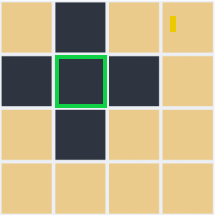
\includegraphics[scale=0.67]{images/4x4_press.PNG}
        % \sethebrew
    \end{subfigure}%
    \begin{subfigure}{.3\textwidth}
        % \unsethebrew
        \caption{לוח לאחר שני לחיצות}
        \label{subfig: explain game, next move}
        \centering
        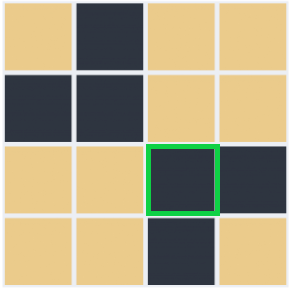
\includegraphics[scale=0.67]{images/4x4_next_press.PNG}
        % \sethebrew
    \end{subfigure}%
\end{figure}
פירוט:
באיור
\ref{subfig: explain game, start}
מתואר מצב התחלתי.
באיור 
\ref{subfig: explain game, move}
ניתן לראות 
את השפעה של לחיצה על משבצת שמסומן בירוק.
באיור
\ref{subfig: explain game, next move}
ניתן לראות השפעה לחיצה נוספת.

לשם הבנה מומלץ לנסות את המשחק,
כפי שנאמר "עדיף לראות פעם אחת, מאשר לשמוע מאה פעמים"
או במקרה שלנו לשחק.
את המשחק אפשר לשחק בקישור הבאה:
\\
\url{https://www.geogebra.org/m/JexnDJpt#chapter/301822}.

האתגר במשחק הוא שאין אסטרטגיה גלויה
לכן, במשחקים רבים מנסים להגיע למצבים שפתרון כבר ידוע.

\subsection{סוגיות בהן נעסוק בפרויקט}
\begin{enumerate}
	\item 
תיאור ודיון בשני אלגוריתמים למציאת פתרון המשחק.
	\item 
הוכחה לקיום פתרון המשחק לכל לוח
	$m\times n$.
	\item 
הרחבה של משחק על לוח למשחק על גרף.
    \item 
נעסוק במספר הפתרון האפשריים בלוח ונדבר על חסם מספר הפתרונות האפשריים.
	\item 
חיפוש לוחות בהם קיים פתרון בו הנורות שינו את מצבם פעם אחת.
    \item 
נציג שיטה למציאת פתרונות בהם כל נורה תשתנה את מצבה פעם אחת.
\end{enumerate}
בנוסף, קיימות שאלות רבות הקשורות למשחק
ובפרויקט ננסה להציג פתרון לחלקן.
יתרה מזאת, נרצה להציג תופעות מעניינות, ולהראות
שהמשחק אינו רק מהנה אלא גם מהווה אתגר מתמטי לא קטן.

\subsection{תיאור משחק על גרף}
אחרי שתיארנו את המשחק על לוח, נתאר את המשחק על גרף.
נזכיר שגרף זה מבנה המכיל קשתות וצמתים, קשתות מוגדרות כצירוף סדור של שני צמתים.
כדי לתאר את משחק האורות על גרף נשתמש באותם כללים שהגדרנו.
במשחק על גרף הצמתים הם המשבצות
לכן, לחיצה על צומת הופכת את מצבה ומצב שכניה.
נגדיר שזוג צמתים יקראו שכנים אם קיימת
קשת המחברת ביניהם.
מטרת המשחק לעבור מגרף שכל הצמתים במצב התחלתי למצב סופי.

\begin{figure}[ht]
    \caption{משחק על גרף לדוגמה}
    \label{fig: start game in graph}
    \begin{subfigure}{.5\textwidth}
        % \unsethebrew
        \centering
        \caption{מצב התחלתי}
        \label{subfig: graph game start}
        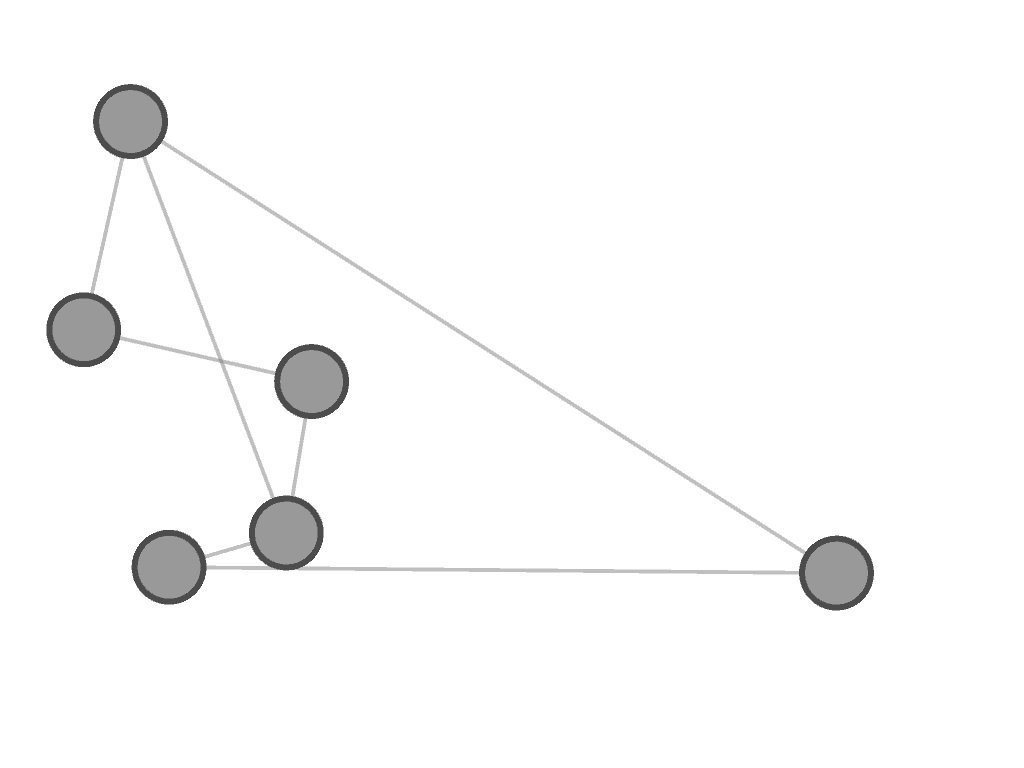
\includegraphics[scale=0.7]{images/graph_start_board.png}
        % \sethebrew
    \end{subfigure}%
    \begin{subfigure}{.5\textwidth}
        % \unsethebrew
        \centering
        \caption{לחיצה על משבצת מסומנת}
        \label{subfig: graph game move}
        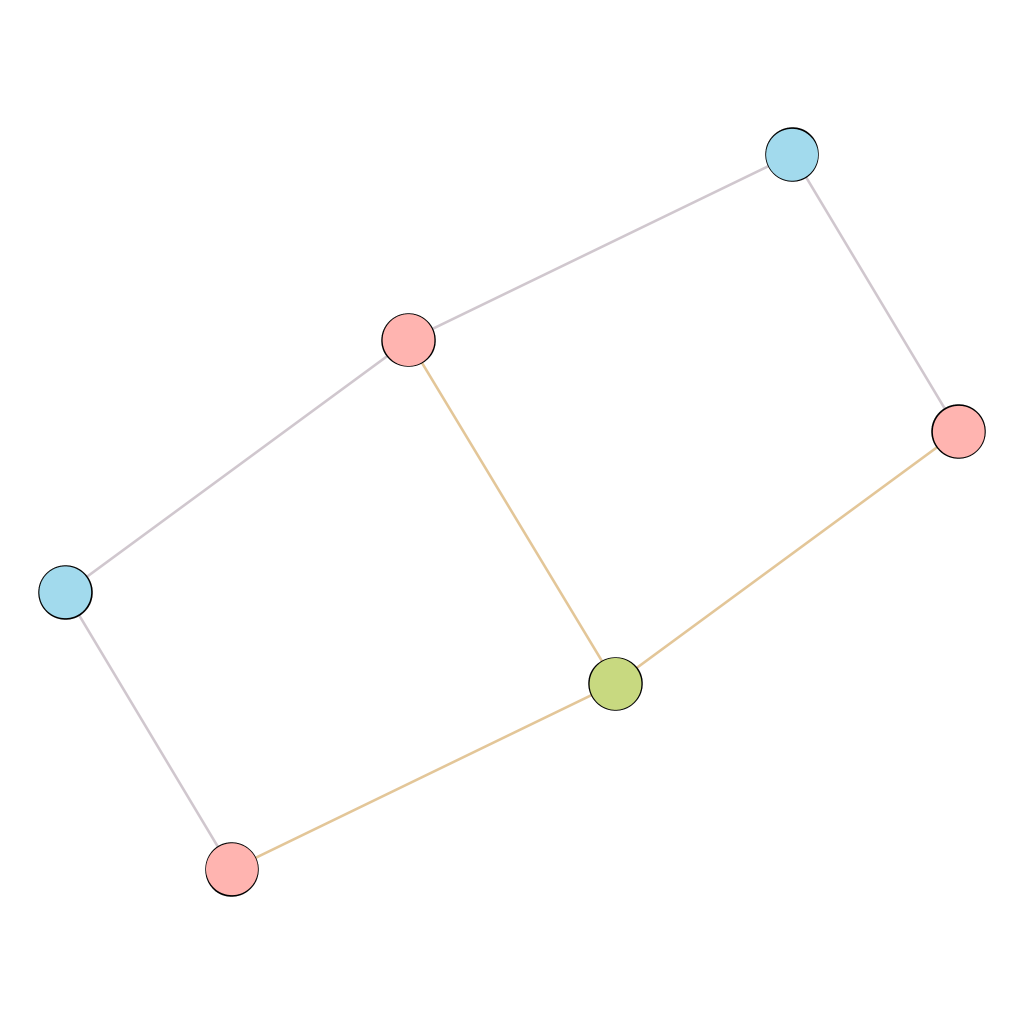
\includegraphics[scale=0.7]{images/graph_press.png}
        % \sethebrew
    \end{subfigure}%
\end{figure}

נמחיש זאת על דוגמה שבאיור
\ref{fig: start game in graph}.
איור 
\ref{subfig: graph game start}
מתאר את מצב התחלתי, נסמן את המצב התחלתי של צומת בצבע כחול.
איור
\ref{subfig: graph game move}
מתאר לחיצה על צומת שצבוע בירוק.
לחיצה זה שינתה את הצמתים השכנות למצבם הסופי שמוסמן בצבע אדום.
\begin{comm}
    בפועל צומת ירוקה גם נצבעת באדום הצביעה לירוק נועדה להצגה.
\end{comm}

\subsection{השוואה בין משחק על לוח למשחק על גרף}
נרצה להראות כי משחק על לוח הוא סוג של משחק על גרף
כלומר, כל משחק על לוח ניתן לתאר בעזרת משחק על גרף.

נתאר משחק על לוח כמשחק על גרף בעזרת הכללים הבאים:
\begin{enumerate}
    \item 
    כל משבצת במשחק על לוח נהפוך לצומת.
    \item 
    כל זוג משבצות סמוכות על לוח נחבר בקשת בגרף.
\end{enumerate}

לדוגמה, ניקח לוח
$2 \times 3$
נמספר את המשבצות כמו באיור
\ref{2x3_board}.
הגרף המתקבל מתואר באיור
\ref{2x3_graph}.

\begin{figure}[ht]
    \caption{
        דוגמה
        למשחק על לוח שתורגם למשחק על גרף
        }
    % \label{fig: start game in graph}
    \begin{subfigure}{.5\textwidth}
        \caption{
            משחק על לוח
            $2 \times 3$
            שמשבצותיו
            ממוספר
        }
        \label{2x3_board}
        % \unsethebrew
        \centering
        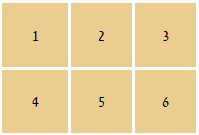
\includegraphics[scale=.95]{images/2x3_board.PNG}
        % \sethebrew
    \end{subfigure}%
    \begin{subfigure}{.5\textwidth}
        \caption{
            משחק על גרף
            שתורגם מלוח
            $2 \times 3$
        }
        % \unsethebrew
        \centering
        \label{2x3_graph}
        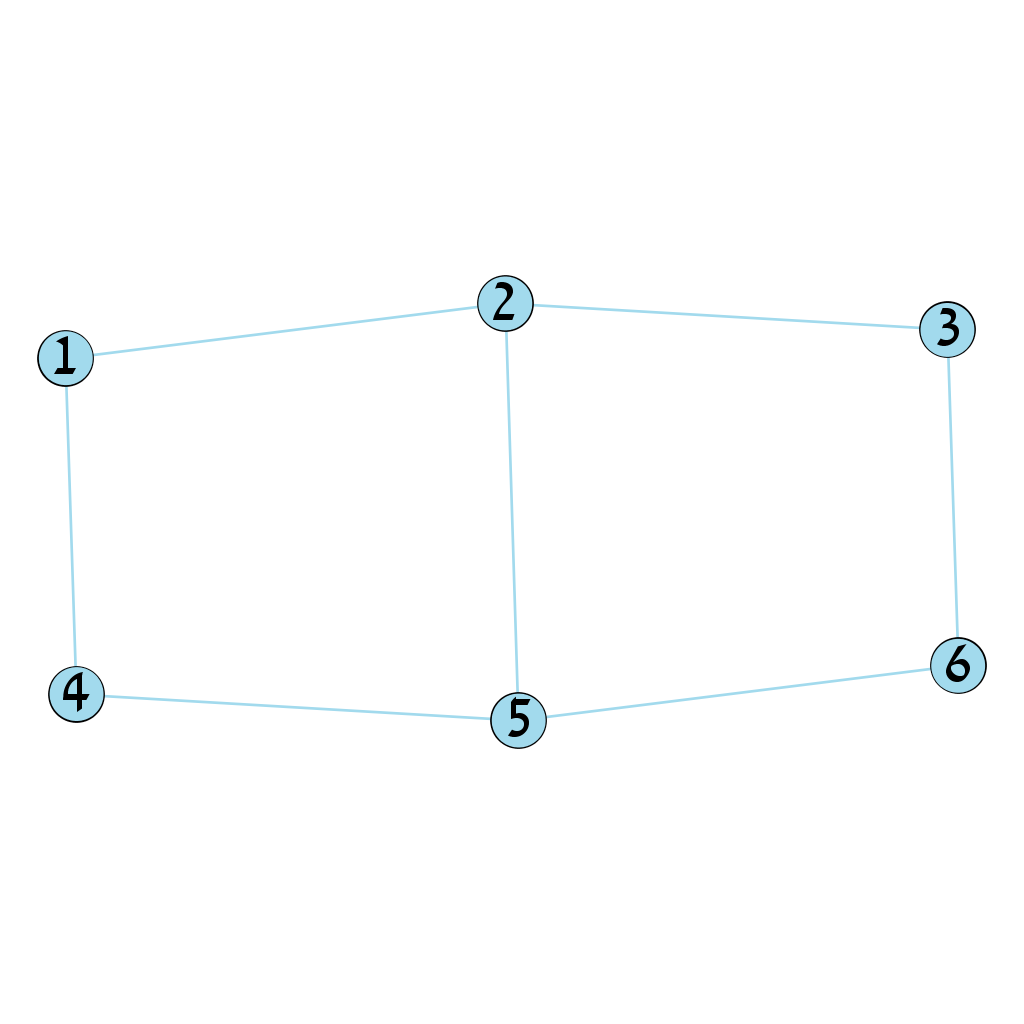
\includegraphics[scale=0.8]{images/2x3_graph.png}
        % \sethebrew
    \end{subfigure}%
\end{figure}

\begin{comm}
קיימים משחקים רבים שניתן לתאר על גרף אך, לא ניתן לתאר אותם על לוח.
לדוגמה, גרף בו יש צומת אם יותר מ
$4$
שכנים לא ניתן לתאר על לוח מכיוון
שלכל
משבצת על לוח
יש לכל היותר
$4$
משבצות סמוכות.
\end{comm}
\begin{comm}
    בעזרת השיטה שתיארנו אפשר לתאר כל משחק על לוח כמשחק על גרף, אבל ההפך הוא לא נכון.
כלומר, לא כל משחק על גרף אפשר לתאר כמשחק על לוח.
\end{comm}
מכיוון שמשחק על לוח ניתן לתאר כמשחק על גרף לכן, טענות שמתקימות
במשחק על גרף נכונות במשחק על לוח.

\newpage

\section{אלגוריתם למציאת פתרון}
לפני שנציג את שיטות למציאת פתרון, נרצה להמחיש את 
האתגר במשחק על ידי הצגה מספר תופעות שמתקיימות במשחק.
באיור
\ref{fig:sol_3_4_5}
מוצגים מספר פתרונות אפשריים ללוחות שונים, לחיצה על הלחצנים הירוקים
בסדר כלשהו תוביל לפתרון המשחק.
ניתן לראות שמספר הלחיצות הנדרשות לפתרון לוח
$4 \times 4$
קטן ממספר הלחיצות הנדרשות לפתרון לוח
$3 \times 3$.
אפשר היה לחשוב שככל שהלוח גדול יותר נדרשות יותר לחיצות 
כדי להגיע לפתרון,
אך, ניתן לראות באיור
\ref{fig:sol_3_4_5}
זה לא נכון.
תופעה נוספת המתקיימת במשחק היא שכמות הפתרונות עבור לוחות שונים משתנה.
עבור לוח 
$3 \times 3$
קיים פתרון יחיד,
אולם ללוח 
$4 \times 4$
קיימים
$16$
פתרונות.
באופן מפתיע, ללוח 
$5 \times 5$
קיימים רק 
$4$.
תופעה זה מפתיע משום שאפשר היה לצפות שככל שהלוח גדול יותר
כך, מספר הפתרונות יגדל.
על מנת לחדד תופעה זו, נסתכל על לוחות ריבועים 
($n \times n$).
נשאל מהו המימד של הלוח אם הכי הרבה פתרונות ומהו מספר פתרונות ללוח זה כאשר
$n \in [1,20]$?
התוצאה המתקבלת היא שמספר הפתרונות הגדול ביותר הוא כאשר
$n = 19$ 
ומספר הפתרונות הוא
$65,536$.
בנוסף
$n = 19$ 
הוא הלוח היחיד ב
$n \in [1,20]$
המקבל את מספר פתרונות זה.
לאומת זאת
מספר הפתרונות השני בגודלו הוא
$256$
ומתקיים בעבור
$n \in \{9, 16 \}$.

\begin{figure}[ht]
    \caption{פתרונות של משחק על לוחות שונים}
    % \unsethebrew
    \label{fig:sol_3_4_5}
    \centering
    \begin{subfigure}[b]{.25\linewidth}
    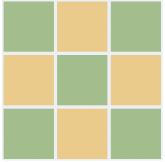
\includegraphics[width=0.95\linewidth]{images/3x3_sol.PNG}
    \end{subfigure}
    \begin{subfigure}[b]{.25\linewidth}
    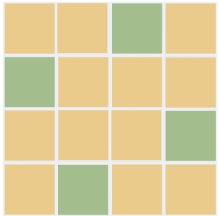
\includegraphics[width=0.97\linewidth]{images/4x4_sol.PNG}
    \end{subfigure}
    \begin{subfigure}[b]{.25\linewidth}
    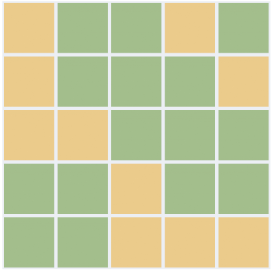
\includegraphics[width=0.95\linewidth]{images/5x5_sol.PNG}
    \end{subfigure}
\end{figure}

שתי גישות למציאת פתרון שנציג בעבודה מבוססות
על מידול הבעיה לשדה לינארי ולמערכת משוואות שפתרונה יוביל לפתרון המשחק.
נתאר את השיטות אומנם, בתחילה הן נראות שונות אך,
נציג את הקשר בינהן.

\newpage
\subsection{אלגוריתם שמבוסס על מטריצת שכנויות}
כדי למדל את הבעיה על שדה לינארי
נשתמש ביצוג גרפי, לחיצה על צומת משנה את הצומת ושכנותיה.
נסמן את צמתים ב
$n_i$.
ניתן לתאר את המשחק בעזרת תיאור אלגברי:
\begin{enumerate}
    \item 
כל צומת יכול להיות בשbי מצבים,
את המצבים נסמן:
    $\{0,1\}$.
    \item 
מצב של צומת 
    $i$
נסמן ב
    $n_i$.
    \item 
המצב התחלתי של משחק על גרף הוא שכל צמתים אם הערך התחלתי
שהוא 
$0$.
    \item 
מצב סופי של משחק
על גרף הוא שכל צמתים 
אם הערך הסופי
שהוא
$1$.
\end{enumerate}
\begin{comm}
    עבור משחקים על לוח נתאר את המשבצות ומצבם הנוכחים ב
    $a_{i,j}$.
    זאת מכיוון שמשחק על לוח ניתן לתאר בעזרת מטריצה.
\end{comm}
\begin{comm}
\label{comm: sum as press operator on board}
פעולת לחיצה על לחצן משנה 
את מצב המנורה,
שינוי מצב מנורה ניתן לתאר בעזרת חיבור בשדה 
$\mathbb{Z}_2$.
נורה שמצבה התחלתי הוא
$n_i$
לאחר לחיצה תעבור למצב
$n_i + 1$.
\end{comm}
תיאור של משחק שכזה מאפשרת לנו
לתאר המשחק בצורה וקוטרית.
אם ניקח לדוגמה
משחק בגודל
$2 \times 2$
נמספר את 
שורות ואז עמודות מלמעלה למטה כמו שמתואר באיור
\ref{fig:numbering_board_2x2}.
נוכל לתאר את הלוח 
שכזה במצבו התחלתי כמטריצה
\[\begin{bmatrix}
0 & 0 \\
0 & 0 
\end{bmatrix}\]
ואם נרצה לתאר את לוח ממצב התחלתי לאחר לחיצה על משבצת 
$1$.
\[ 
    \begin{bmatrix}
    0 & 0 \\
    0 & 0 
    \end{bmatrix} \stackrel{n_1}{\longrightarrow}
    \begin{bmatrix}
    1 & 1 \\
    1 & 0 
    \end{bmatrix}
 \]
 כפי שתיארנו 
 בהערה 
 \ref{comm: sum as press operator on board}
 אפשר לתאר שינוי מצב הנורה על ידי חיבור 
 עם אחד.
\[
    \begin{bmatrix}
    0 & 0 \\
    0 & 0 
    \end{bmatrix} + 
    \begin{bmatrix}
    1 & 1 \\
    1 & 0 
    \end{bmatrix}=
    \begin{bmatrix}
    1 & 1 \\
    1 & 0 
    \end{bmatrix} 
\]  
 אם נציג כל מטריצה ע"י ווקטור קואורדינטות בסיס סטנדרטי של מרחב מטריצות אז נוכל לרשום את השוויון הנ"ל גם כך
 \[ 
    \begin{bmatrix} 
    0 \\ 0 \\ 0 \\ 0
    \end{bmatrix} +  \begin{bmatrix} 
    1 \\ 1 \\ 1 \\ 0
    \end{bmatrix} =  \begin{bmatrix} 
    1 \\ 1 \\ 1 \\ 0
    \end{bmatrix}  
 \]
וקטור שחיברנו עם מצב הלוח התחלתי הוא וקטור שמתאר את הלחיצה ונקראה לו בעבודה זה וקטור שינוי.
 \begin{definition}
    תהי 
    משחק על גרף בעל
    $n$
    צמתים
    ממספרים מ
    $1$
    עד
    $n$,
    וקטור שינוי
    $t_i$
    של צומת  
    $i$
    הוא 
    וקטור 
    שייך 
    $\Zn$,
    שאם תחבר אותו אם מצב הלוח הנוכחי 
    התוצאה המתקבלת תהיה מצב הלוח 
    לאחר לחיצה על צומת 
    $i$.
\end{definition}
כדי לבנות וקטור שינו 
של 
צומת 
$i$
נשים ערך 
$1$
בכל אינדקסים 
בהם האינדקס שווה 
למספור 
של 
צומת 
שכנה
לצומת
$i$
ובאינדקס של צומת עצמה
כלומר,
באינדקס 
$i$.
שאר הערכי הוקטור הם אפס.

\begin{figure}[ht]
    \caption{שיטת מספור משבצות על לוח}
    \label{fig:numbering_board_2x2}
    % \unsethebrew
    \centering
    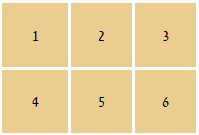
\includegraphics[width=0.3\textwidth,keepaspectratio]{images/2x3_board.PNG}
\end{figure}

\begin{comm}
    \label{ comm: indexing board game}
    מספור לוח שעובר על שורות ואז עמודות מלמעלה למטה כמו שמתואר באיור
    \ref{fig:numbering_board_2x2},
     היה שיטת המספור הקבוע בפרויקט זה עבור משחקים על לוח.
\end{comm}
נדגים על גרף תיאור וקטורי השינוי,
נבצע זאת על גרף באיור
\ref{fig: change vector on graph}.
באיורים עלו נצבע אדום צמתים שמצבם  
$1$
ובכחול 
צמתים שמצבם 
$0$.
בעזרת וקטור השינוי אפשר לתאר תוצאה של מספר לחיצות,
נעשה זאת בעזרת חיבור וקטור שינויים
וחיבור מצב הגרף.
התוצאה שנקבל 
תהיה הגרף המתקבל לאחר לחיצה של צמתים
הללו.
נדגים רעיון זה כאשר מצב של גרף מתואר באיור
\ref{fig:start graph presses}.
נניח שצומת 1 היא יחידה שדלוקה.
נרצה להראות איך הגרף יראה אם ילחצו על כפותרים 
$1, 3$.
וקטור שינוי של צומת 
$1$
הוא
\[
    t_1 = 
    \begin{bmatrix}
        1 \\
        0 \\
        1 \\
        1 \\
    \end{bmatrix}
\]
\[
    t_1 + t_3 = 
    \begin{bmatrix}
        1 \\
        0 \\
        1 \\
        1 \\
    \end{bmatrix}
    +
    \begin{bmatrix}
        1 \\
        1 \\
        1 \\
        1 \\
    \end{bmatrix}
    =
    \begin{bmatrix}
        0 \\
        1 \\
        0 \\
        0 \\
    \end{bmatrix}
\]
ומצב התחלתי שמתואר באיור נסמן ב
$S_0$
לכן מתקבל
\[
    S_0 + t_1 + t_3 = 
    \begin{bmatrix}
        1 \\
        0 \\
        0 \\
        0 \\
    \end{bmatrix}
    +
    \begin{bmatrix}
        0 \\
        1 \\
        0 \\
        0 \\
    \end{bmatrix}
    =
    \begin{bmatrix}
        1 \\
        1 \\
        0 \\
        0 \\
    \end{bmatrix}
\]
הגרף המתקבל לאחר חיבור אכן תואם לתוצאה המצופה
מתואר באיור 
\ref{fig:start graph presses solution}.

\begin{figure}[ht]
    \caption{
        דוגמה לתיאור וקטור שינוי במהלך משחק על גרף
        }
    \label{fig: change vector on graph}
    \centering
    \begin{subfigure}[b]{.4\linewidth}
        \caption{מצב של הגרף לפני לחיצה}
        \label{fig:start graph presses}
        % \unsethebrew
        \centering
        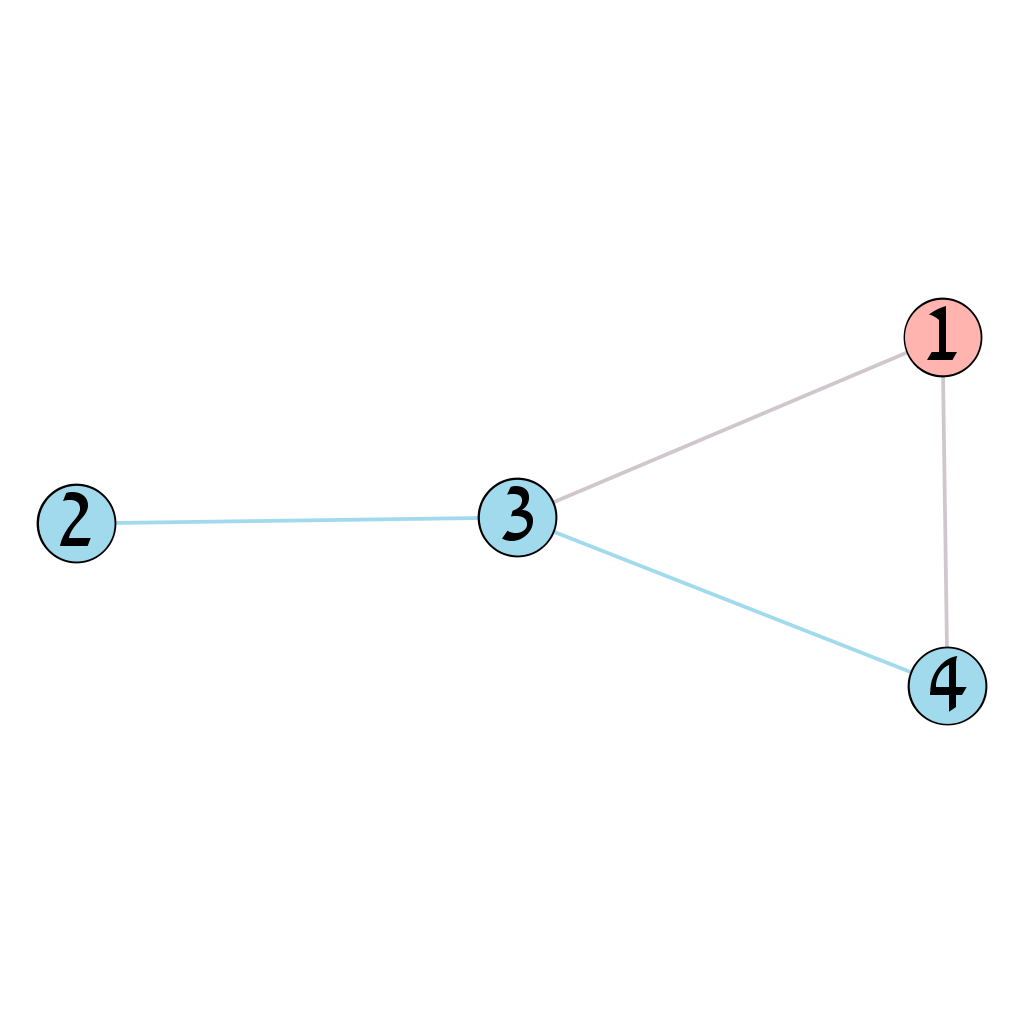
\includegraphics[width=.7\textwidth,keepaspectratio]{images/graph_presses.png}
    \end{subfigure}
    \begin{subfigure}[b]{.4\linewidth}
        \caption{מצב של הגרף לפני לחיצה}
        \label{fig:start graph presses solution}
        % \unsethebrew
        \centering
        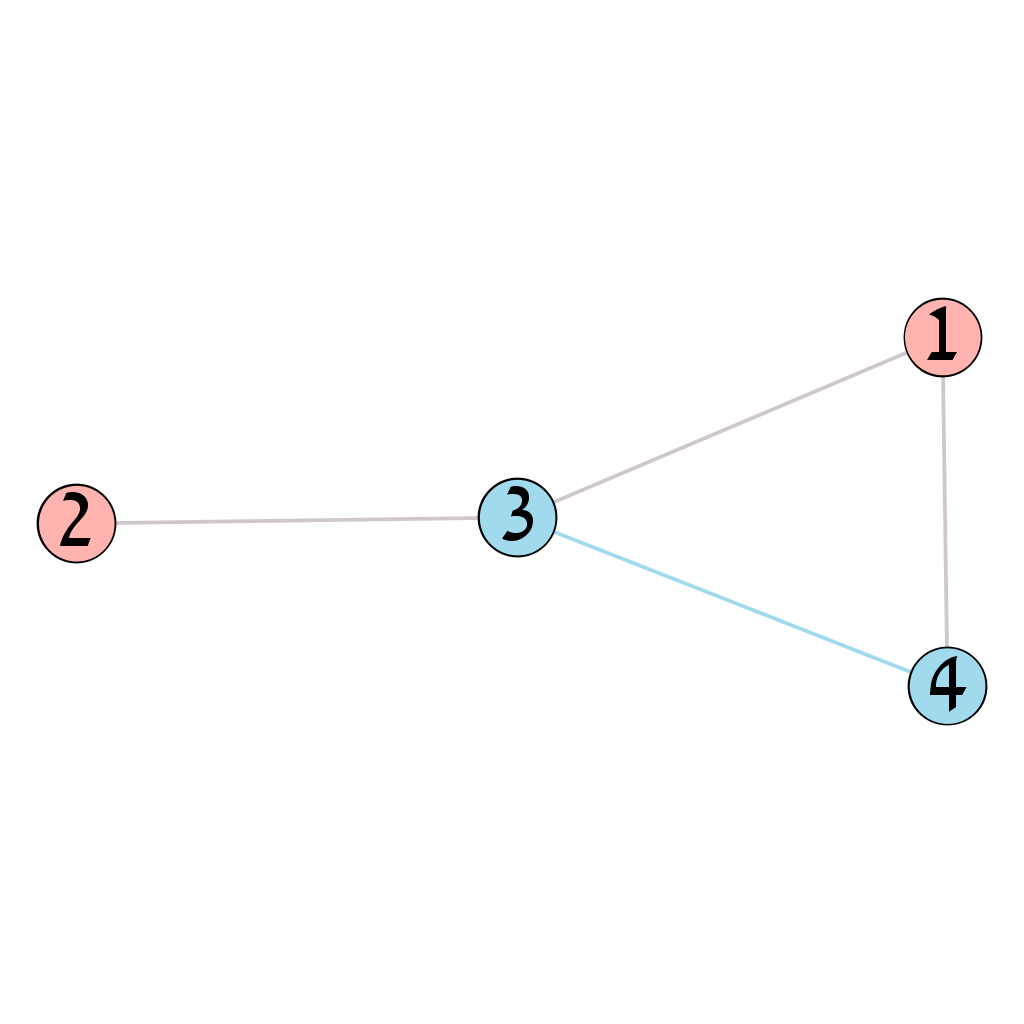
\includegraphics[width=.7\textwidth,keepaspectratio]{images/graph_presses_solve.png}
    \end{subfigure}
\end{figure}

\begin{comm}
    היות ווקטור שינוי שדה
    $\Zn$
    חיבור בין וקטורים הינו חיבור בין האינדקסים מודולו 
    $2$
    וכפל בסקלר
    הוא לכפול את כל ערכי וקטור בסקלר
    כאשר הסקלרים יכולים להיות
    $0$
    או 
    $1$
\end{comm}
\begin{comm}
    מספר זוגי של לחיצות אינו משנה את מצב הלוח
\end{comm}
היות 
ואנחנו עובדים על שדה מודולו 
$2$
$t_i + t_i = \vec{0}$.
\begin{comm}
    \label{comm: press is uneven presses}
    לא משנה כמה תלחץ על לחצן בודד הלחצן 
    יכול להעביר אותך לשני מצבים שונים בלוח.
\end{comm}
מספר הלחיצות על אותו לחצן אינו משנה 
לחצן עכשיו 
לחוץ אם נלחץ מספר אי זוגי של פעמים 
כי מספר לחצות הזוגיות לא שינו את הלוח.
בנוסף זה מסביר את הסיבה למה כפל בסקלר שאנחנו מוכנים לקבל הוא הערכים 
$0,1$.
לכן בהמשך
הפתרון יתואר אם יש צורך ללחוץ בלחצן או לא,
לא תהיה התייחסות לכמות הלחיצות כי התוצאה מתקבלת רק תלויה בזוגיות של מספר הלחיצות.
\begin{comm}
    היות ומצב התחלתי הוא שכל הצמתים 
    במצב 
    $0$
    לכן,
    ניתן לתאר 
    את המצב עליו נעבור
    רק
    בעזרת צירוף לינארי של וקיטורי שינוי בלבד.
\end{comm}
היות ומצב התחלתי נסמן כרגע ב
$S_0$
הוא כולו וקטור האפס
מתקיים:
\begin{equation}
    \label{eq: sum change vectors}
    S_0 + \sumi{j} \vec{t_j} x_j=  \sumi{j}  \vec{t_j}x_j
\end{equation}
בעקבות כך ניתן לתאר את בעיית המשחק לצורה הבאה:
\begin{equation}
    \label{eq: lin eq for solving problem}
    \sumi{j} \vec{t_j} x_j = \vec{1}
\end{equation}
כאשר
$\vec{1}$
וקטור שכל ערכיו אחדים,
שזהו מצב הסופי של הגרף
ו
$n$
מספר הצמתים בגרף.
נשים לב 
שאם 
ידוע צירוף
$x = \begin{bmatrix}
    x_1, & x_2, & \cdots , x_n
\end{bmatrix}$
שמקיים את המשוואה 
\ref{eq: lin eq for solving problem}
קיבלנו פתרון של משחק על גרף.
כדי להגיע לפתרון על גרף נלחץ על הצמתים שמספורם 
שווה 
לאינדקסים 
שמקיימים
$x_j = 1$
בצירוף 
$x$.

בנוסחה
\ref{eq: sum change vectors}
קיימים מספר תכונות 
שנרצה לציין.
\begin{lemma}
    \label{lemma: order presses}
    סדר הלחיצות לא משנה את התוצאה הסופית
\end{lemma}
בגלל אסוציאטיביות של חיבור בשדה 
סדר לחיצות לא משנה.
\begin{lemma}
    \label{lemma: num presses}
    כמות האפשרויות לחיצה על לוח
    $m \times n$
    הוא 
    $2^{m \cdot n}$
\end{lemma}
לפי הערה 
\ref{comm: press is uneven presses}
כל לחצן יכול להיות בשתי מצבים 
והיות לפי
למה
\ref{lemma: order presses}
סדר הלחיצות לא משנה,
לכן ללוח
$m \times n$
מספר אפשרויות לחיצה 
$2^{m \cdot n}$.
כדי להבין גודל מספר זה נסתכל במשחק על לוח 
$6 \times 6$
כמות  אפשרויות לחיצה גדולה 
מכמות הסטנדרטית שמציגים מספר שלמים,
$4$
בתים
כלומר המספר הגדול ביותר שאפשר להציג  בעזרת 
$4$
בתים
הוא
$2^{32}-1$
המטרה של המחשה זה להדגיש כמה לא פרקטית לנסות לפתור בעזרת
ניסיון כל האופציות האפשריות.

מערכת משוואות 
שמתוארת בנוסחה
\ref{eq: lin eq for solving problem}
אפשר לתאר במספר צורות.
נפוצה מבניהם היא
בעזרת מטריצה כמו שמתואר 
בנוסחה 
\ref{eq: matrix eq for solving problem}.
\begin{equation*}
    \begin{bmatrix}
        t_1 & t_2 & \cdots & t_n
    \end{bmatrix}
    \begin{bmatrix}
        x_1 \\
        x_2 \\
        \cdots \\
        x_n \\
    \end{bmatrix}
    =
    \begin{bmatrix}
        1 \\
        1 \\
        1 \\
        1 \\
    \end{bmatrix}
\end{equation*}
\begin{equation}
    \label{eq: matrix eq for solving problem}
    \begin{bmatrix}
        t_{1,1} & t_{1,2} & \cdots & t_{1,n} \\
        t_{2,1} & t_{2,2} & \cdots & t_{2,n} \\
        \cdots & \cdots & \cdots & \cdots\\
        t_{i,j} & t_{i,2} & \cdots & t_{i,n} \\
        \cdots & \cdots & \cdots & \cdots\\
        t_{n,1} & t_{n,2} & \cdots & t_{n,n} \\
    \end{bmatrix}
    \begin{bmatrix}
        x_1 \\
        x_2 \\
        \cdots \\
        x_n \\
    \end{bmatrix}
    = 
    \begin{bmatrix}
        1 \\
        1 \\
        \cdots \\
        1 \\
    \end{bmatrix}
\end{equation}
נשים לב שלמטריצה
$A$
במשוואה
\ref{eq: matrix eq for solving problem}
מתקבל ש
$A_{i,j} = 1$
כאשר 
$i, j$
צמתים שהם שכנים או זהים
$i = j$.
\begin{definition}
    \label{def: neighbor matrix}
    מטריצה שמתארת את משחק 
    שקבלנו במשוואה
    \ref{eq: matrix eq for solving problem}
    תקראה מטריצת שכנויות של משחק.
\end{definition}
\begin{comm}
    \label{comm: symetic matrix}
    היות וכל צומת שכנה היא שכנה אחד לשני לכן במטריצה
    סימטרית
\end{comm}
דוגמה למטריצה  המתקבלת מגרף באיור 
\ref{fig:start graph presses solution}:
\[
    \begin{bmatrix}
        1 & 0 & 1 & 1\\
        0 & 0 & 1 & 0\\
        1 & 1 & 1 & 1\\
        1 & 0 & 1 & 1\\
    \end{bmatrix}
\]
\begin{definition}
    \label{ def: solution vector}
    תהי משחק ומערכת משוואת שמתארת אותו מצורה 
    \ref{eq: matrix eq for solving problem} 
    נגדיר את וקטור פתרון כצירוף הערכים מביאים לפתרון
    של מערכת המשוואות
    ונסמן אותו ב
    $\vec{x}$
\end{definition}
נזכיר שאם
$\vec{x}$
וקטור פתרון של המערכת 
ו
$x_i = 1$
אז המשמעות שכדי לפתור את המשחק
צריך ללחוץ על לחצן 
$i$.
בנוסף 
נזכיר שאתכן שהיו כמה פתרונות אפשריים.
\begin{definition}
    \label{def: standard solution}
    שיטת פתרון בעזרת יצירת  מטריצה שכנויות על ידי וקטור שינויים תקראה
    אלגוריתם מבוסס מטריצת שכנויות.
\end{definition}
תוצאה דומה
לתיאור שיטת הפתרון מבוססת מטריצת השכנויות 
אפשר לראות מהספר
\cite{B2}.
מרגע שהצלחנו לתאר את הבעיה מערכת משוואות לינארית
על שדה
$\Zn$
מכן נוכל להיעזר בכלים של אלגברה לינארית כדי למצוא את הפתרון כמו מציאת פתרון בעזרת דירוג,
מציאת מטריצה פסאודו הפוכה וכולי. 
\begin{comm}
    \label{comm: for board too many variables}
    עבור משחק על לוח 
    $m \times n$
    גודל מערכת המשוואות המתקבל משיטה 
    מבוססת מטריצת שכנויות 
    הוא 
    $m \cdots n$
    משתנים ומשוואות.
\end{comm}
עבור לוח 
$[m \times n]$
כמות הלחצנים 
$m \cdot n$
ולכן 
קיבלנו גודל שכזה.
השאלה הטבעית שעולה האם אפשר לצמצם את גדול זה?

\subsection{אלגוריתם שמבוסס על מילוי עקבי של שורות}
עד כה
הצגנו
בעבודה
גישה פתרון
הנעזרת במטריצת שכנויות,
נרצה להראות שיטה נוספת למציאת פתרון.
שיטת הפתרון שנציג נובעת מהערה 
\ref{comm: for board too many variables}
נרצה להציע שיפור ולצמצם את כמות המשתנים והמשוואות 
למציאת פתרון למשחק על לוח 
$ m \times n$
ב
$\min(m,n)$
משוואות ומשתנים.
צמצום גודל המערכת המשואות יכולה להוביל לחישוב מהיר יותר וניצול טוב יותר של מידע.

המאמר 
\cite{B1}
מציג שיטה למציאת פתרון
של משחק על לוח כלשהו,
בגישה קצת שונה.
בפרק זה נציג את הגישה שמתוארת 
\cite{B1}
ונראה את הקשר של בין שתי השיטות.
לגישה החדשה ניקרא לאורך כל הפרק שאלגוריתם שמבוסס על מילוי עקבי של שרות
או בקצרה מילוי עקבי.
\begin{definition}
    \label{def: spanish way}
    שאלגוריתם שמבוסס על מילוי עקבי של שרות, היא שיטה שמבוססת על עיקרון 
    שאם, ידוע איזה כפתורים צריכים להילחץ בשורה העליונה כדי להגיע לפתרון, אפשר לגלות את כל שאר הכפתורים שצריכים להילחץ 
    כמעט מידית.
\end{definition}
נתאר את 
שאלגוריתם שמבוסס על מילוי עקבי של שרות
בשלבים,
כל שלב נדגים
על לוח 
$3 \times 3$
שמתואר באיור 
\ref{fig: 3 x 3 board indexed}.
הלוח 
$3 \times 3$
הנתון ממספור באינדקסים 
בשיטה דומה כפי שתיארנו בהערה 
\ref{ comm: indexing board game}.
שאלגוריתם שמבוסס על מילוי עקבי של שרות
מתבסס על רעיון,
שפתרון של המשחק הוא סדרה של לחיצות על משבצות מסוימות. נשייך
 לכל משבצת משתנה שיכול לקבל שני ערכים: 
 $0$
  אם משבצת הזאת מופיעה בסדרת לחיצות של פתרון
 ו-
 $1$
 אם משבצת הזאת כן מופיעה בסדרת לחיצות של פתרון המשחק.
  מראש לא ידוע לנו
 האם משבצות של שורה ראשונה יופיעו בסדרה הזאת או לא. אז משתנים של משבצות בשורה ראשונה
 עבור
 איור 
 \ref{fig: 3 x 3 board indexed}
 הם
 $x_1, x_2, x_3$.

\begin{figure}[ht]
    \caption{לוח 
    $3 \times 3$
    עם אינדקסים}
    \label{fig: 3 x 3 board indexed}
    % \unsethebrew
    \centering
    \[\begin{bmatrix}
        x_1 & x_2 & x_3 \\
        x_4 & x_5 & x_6 \\
        x_7 & x_8 & x_9 \\
    \end{bmatrix}    
    \]
\end{figure}

נבחין בתופעה הבאה,
על מנת שהנורה במשבצת ראשונה בשורה ראשונה תהיה דולקת סכום המשתנה שלה 
ומשתנים של משבצות השכנות במודולו
$2$ 
חייב להיות 
$1$. 
המשוואה המתקבלת עבור איור 
\ref{fig: 3 x 3 board indexed}:
\begin{equation}
    \label{eq: cond eq}
    x_1 + x_2 + x_4 = 1  
\end{equation}
לכן משתנה 
במשבצת ראשונה בשורה שניה,
שסימנו במשתנה 
$x_4$
חייב להיות שווה ל
$x_1 + x_2 +1 $
היות ומתקיים:
\[
    x_1 + x_2 + x_4 = 1 \Rightarrow x_4 = x_1 + x_2 + 1  
\]
על מנת שהנורה במשבצת שנייה בשורה ראשונה
תהיה דולקת סכום 
משתנה שלה ומשתנים של משבצות שכנות במודולו
$2$ 
חייב להיות 
$1$.
לכן מתקבל שערכו של 
$x_5$
חייב להיות שווה ל
$x_1+x_2+x_3+1$
היות ומתקיים:
\[
    x_1 + x_2 + x_3 + x_5 = 1 \Rightarrow x_5 = x_1 + x_2 + x_3 +1
\]
 באופן דומה מחשבים ערכי משתנים של שאר המשבצות בשורה שנייה ואחר כך
 על פי אותם שיקולים ערכי משתנים של משבצות בשורות הבאות. 
 \begin{figure}[ht]
    \caption{
        תרגום כל הלחצנים לפי המשתנים של השורה העליונה
    }
    \label{fig: 3 x 3 board fill intire board}
    % \unsethebrew
    \centering
    \[
    \begin{bmatrix}
        x_1 & x_2 & x_3 \\
        1 + x_1 + x_2 & 1 + x_1 + x_2 + x_3 & 1 + x_2 + x_3 \\
        1 + x_1 + x_3 & 0 & 1 + x_1 + x_3 \\
    \end{bmatrix}
    \]
\end{figure}
נבחין שלאחר שמילאנו את כל הלוח כמו שמתואר באיור 
\ref{fig: 3 x 3 board fill intire board}.
אם היה ידוע איזה לחצנים משורה העליונה שייכים לסדרת הלחיצות של פתרון אז, פתרנו את המשחק.
\begin{definition}
    \label{ def: depndeciy equation}
    המשוואה של סכום
    משתנים של משבצת  
    $i$
    וכל שכניה
    תקראה
    משוואת אילוצים על לחצן 
    $i$
\end{definition}
משוואה 
\ref{eq: cond eq}
הינה משוואת האילוצים שללחצן
$4$.
עבור משחק לוח
ריבועי באורך שורה 
$n$
שהלחצנים ממספרים לפי הערה
\ref{ comm: indexing board game}
ניתן לנסח בנוסחה פשוטה:
\begin{equation}
    \begin{english}
    \label{eq: depndeciy equation}
    x^*_{i - n} + x^*_{i - 1} + x^*_{i} + x^*_{i + 1} + x^*_{i + n} = 1
    \hspace{10pt}
    x^*_i =
    \begin{cases}
        x_i & \text{if } i \in [1,n \cdot m]
        \\
        0 & \text{otherwise}
    \end{cases}
    \end{english}
\end{equation}
נדגים חישוב
משתנה לא משורה השנייה,
העליונה ביותר,
נתאר את
$x_7$
בעזרת משתנים משורה העליונה.
היות ו-
$x_7$
משורה שלישית לכן נצטרך 
שהמשתנים מהשורה שניה בוטאו בעזרת משתנים משורה העליונה.
נחלץ את 
$x_7$
ממשואת האילוצים של לחצן
$4$
שזה הלחצן שמעליו.
\[ x_1 + x_4 + x_5 + x_7 = 1 \]
לכן 
\[ x_7 = 1 + x_1 + x_4 + x_5  \]
היות ושמשתנים משורה השנייה הוגדרו לפי משתנים 
משורה העליונה:
\begin{align*}
    x_4 &= 1 + x_1 + x_2 \\
    x_5 &= 1 + x_1 + x_2 + x_3
\end{align*}
נציב ערכים אילו
\begin{equation*}
    x_7 = 1 + x_1 + (1 + x_1 + x_2) + (1 + x_1 + x_2 + x_3) \Rightarrow
    x_7 = 1 + x_1 + x_3
\end{equation*}
על מנת ליצור מערכת משוואות
שתפתור את המשחק
מחבר המאמר
\cite{B1}
מוסיף לשורה האחרונה עוד שורה, שורה דמיונית ומחשב ערכי 
משתנים של המשבצות שלה לפי אותם שיקולים.
\begin{figure}[ht]
    \caption{לוח 
    $3 \times 3$
    מלאה
    כולל שורה וירטואלית
    }
    \label{fig: 3 x 3 board fill with virtual}
    \centering
    \[
        \begin{bmatrix}
            x_1 & x_2 & x_3 \\
            1 + x_1 + x_2 & 1 + x_1 + x_2 + x_3 & 1 + x_2 + x_3 \\
            1 + x_1 + x_3 & 0 & 1 + x_1 + x_3 \\
            \hline
            1 + x_2 + x_3 & x_1 + x_2 + x_3 & 1 + x_1 + x_2 \\
        \end{bmatrix}
    \]
\end{figure}
משום שזאת שורה דמיונית, 
בעצם אנחנו לא מדליקים אף נורה בה ערכי המשתנים של משבצות
שלה חייב להיות אפס.
כך נוצרת מערכת משוואות עם 
$n$
משוואות ו- 
$n$
משתנים וזה ההסבר שנתן מחבר המאמר.
\begin{figure}[ht]
    \caption{
        מערכת המשואות המתקבלת משיטה פתרון לפי שורה העליונה
        בלוח 
        $3 \times 3$
    }
    \label{fig: eq system for spanish method 3 x 3}
    
    \[\begin{cases}
        1+x_{1}+x_{2}=0\\
        x_0 + x_1 + x_2 = 0\\
        1 + x_0 + x_1 = 0
        \end{cases} \]
\end{figure}

את השיטה הדגמנו על לוח 
$3 \times 3$,
אפשר היה להדגים על כל לוח ושיטה תעבוד.
בנוסף, שיטה שתיארנו ביצע מעבר על שורות אפשר היה לעשות בניה דומה גם לעמודות.
בגלל שאפשר להפעיל את השיטה על שורות או עמודות 
כדי לקבל מערכת משוואות קטנה ביותר נבחר 
את כיוון עם פחות משבצות.
המאמר 
\cite{B1}
מתאר מספר רב של פתרונות  בלוחות ריבועים בגדלים שונה ואפילו על לוחות מלבניים.
האתגר המרכזי בשיטה הספרדית היא להצדיק אותה למה יש שורה וירטואלית
והאם יש קשר בין שני השיטות.
בשלב זה נתרכז להראות את הקשר בין שיטה הספרדית ושיטה שהצגנו בפרק הקודם.
\begin{theorem}
    מטריצה המיצג של מערכת המשוואות האילוצים היא מטריצת שכנויות
\end{theorem}
משוואות האילוצים היא כל מהות של האלגוריתם למילוי עקבי
מכיוון שהתקדמות בשורות מבוססת על המשוואות עלו.
אם נפרוס את משוואת האילוצים נקבל גם מערכת משוואת שפותרת את המשחק
אבל כמות המשואות הינה 
$n^2$.
נבחין שאם נציג אותם כמטריצה כאשר כל משוואת אילוצים מסודר לפי סדר הלחצנים נקבל את מטריצה שכנויות.

נדגים זאת על לוח 
$2 \times 2$
שמתואר באיור
\ref{fig: 2 x 2 board}.
\begin{figure}[ht]
    \caption{לוח 
    $2 \times 2$
    }
    \label{fig: 2 x 2 board}
    % \unsethebrew
    \centering
    \[
        \begin{bmatrix}
            x_1 & x_2 \\
            x_3 & x_4 \\
        \end{bmatrix}
    \]
\end{figure}
וקטור השינויים:
\[
   t_0 = 
    \begin{bmatrix}
        1 \\
        1 \\
        1 \\
        0 \\
    \end{bmatrix},
    t_1 = 
    \begin{bmatrix}
        1 \\
        1 \\
        0 \\
        1 \\
    \end{bmatrix},
    t_2 = 
    \begin{bmatrix}
        1 \\
        0 \\
        1 \\
        1 \\
    \end{bmatrix},
    t_3 = 
    \begin{bmatrix}
        0 \\
        1 \\
        1 \\
        1 \\
    \end{bmatrix},
\]
לכן
מטריצת שכנויות נראת כך:
\[
    \begin{bmatrix}
        1 & 1 & 1 &0 \\
        1 & 1 & 0 & 1 \\
        1 & 0 & 1 & 1 \\
        0 & 1 & 1 & 1 \\
    \end{bmatrix},
\]
אם נסדר את המשוואות במערכת המשוואות לפי סדר 
האינדקסים של המשבצות נקבל את המערכת מהצורה
\begin{align*}
    x_0 + x_1 + x_2 &= 1\\
    x_0 + x_1 + x_3 &= 1\\
    x_0 + x_2 + x_3 &= 1\\
    x_1 + x_2 + x_3 &= 1
\end{align*}
אפשר לראות שאם נבנה את המטריצה המייצגת של המערכת נקבל מטריצה דומה למטריצת השכנויות.

תעלומה נוספת שנסנה לפתור באלגוריתם למילוי עקבי היא למה צריך שורה וירטואלי, למה ערכה 
שווה ל
$0$,
וכיצד באמת מתבצע צמצום כמות המשתנים ל
$n$
משתנים.
הסבר לתופעה זה
ניתן בעזרת תיאור אלגוריתם מילוי עקבי רק שהפעם את
הפעולות במקום לעשות על טבלה שתיארה את הלוח, נבצע על המטריצה שמתארת את מערכת המשוואות 
,
מטריצת השכנויות.
נראה את הפעולות שעושים בשיטה על אותה דוגמה 
על לוח 
$3 \times 3$.
 ונרצה להראות שאלגוריתם מילוי עקבי הוא דירג מתוחכם של מטריצה מורחבת 
$[M | \vec{1}]$.

\begin{figure}[ht]
    \caption{
        מערכת משוואות מורחבת של משחק על לוח 
        $3 \times 3$
    }
    \label{fig: full matrix 3 x 3}
    \begin{english}
        \begin{center}
            \[\left[
            \begin{array}{ccccccccc|c}
                    1& 1& 0& 1& 0& 0& 0& 0& 0& 1 \\
                    1& 1& 1& 0& 1& 0& 0& 0& 0& 1 \\
                    0& 1& 1& 0& 0& 1& 0& 0& 0& 1 \\
                    1& 0& 0& 1& 1& 0& 1& 0& 0& 1 \\
                    0& 1& 0& 1& 1& 1& 0& 1& 0& 1 \\
                    0& 0& 1& 0& 1& 1& 0& 0& 1& 1 \\
                    0& 0& 0& 1& 0& 0& 1& 1& 0& 1 \\
                    0& 0& 0& 0& 1& 0& 1& 1& 1& 1 \\
                    0& 0& 0& 0& 0& 1& 0& 1& 1& 1 \\
            \end{array}
            \right]\]
        \end{center}
    \end{english}
\end{figure}

כדי לחשב את 
$x_4$
באיור
\ref{fig: 3 x 3 board indexed}
השתמשנו במשוואת האילוצים של 
משבצת 
$1$,
אשר מתוארת במטריצה בשורה ראשונה.
\[
    x_1 + x_2 + x_4 = 1 \Rightarrow x_4 = x_1 + x_2 + x_3
\]
נבחין שלושת השורות הראשונות  
של המטריצה 
\ref{fig: full matrix 3 x 3}
מאפשרות תיאור פשוט של המשתנים 
$x_4, x_5, x_6$,
בגלל ששורות עלו ניתן לבטא כמשוואות האילוצים של לחצנים 
$1,2,3$
אם ננסה לתאר 
את משתנה 
$x_7$
באותה שיטה 
נסתכל על שורה ה 
$4$
במטריצה 
וניראה שהיא תלויה ב
$x_4, x_5$
היות ואמרנו
שאפשר בקלות לתאר את משתנים עלו 
בעזרת שורות 
$1,2$
במטריצה לכן 
נעזר בשורות עלו כדי לתאר את 
$x_7$,
אופן שימוש בשורות עלו תהיה 
הפעלה פעולה שורות הבאה:
\begin{align*}
    r_4 \leftarrow r_4 + r_1
    \\
    r_4 \leftarrow r_4 + r_2
\end{align*}
שני פעולות שורות הללו הם שקולות לפעולה אלגברית הבאה
:
\begin{align*}
   (x_1 + x_4 + x_5 + x_7 + 1) + (x_1 + x_2 + x_4 + 1) = 0 \Rightarrow x_2 + x_5 + x_7 = 0
    \\
    (x_2 + x_5 + x_7) + (x_1 + x_2 + x_3 + x_5 + 1 ) = 0 \Rightarrow x_1 + x_3 + x_7 + 1 = 0
\end{align*}
ועכשיו קיבלנו תיאור 
של 
$x_7$
בעזרת המשתנים של שורה העליונה.
בכך תרגמנו את אלגוריתם מילוי עקבי בעזרת פעולת שורות על מטריצה מורחבת.
אחרי שנעבור על כל השורות בצורה שכזה נקבל את המטריצה
\ref{fig: matrix after spanish}.
\begin{figure}[ht]
    \caption{המטריצה לאחר פעולת שורות על כל שורות}
    \label{fig: matrix after spanish}
    \begin{english}
        \begin{center}
            \[
                \left[
                \begin{array}{ccccccccc|c}
                1& 1& 0& 1& 0& 0& 0& 0& 0& 1 \\
                1& 1& 1& 0& 1& 0& 0& 0& 0& 1 \\
                0& 1& 1& 0& 0& 1& 0& 0& 0& 1 \\
                1& 0& 1& 0& 0& 0& 1& 0& 0& 1\\
                0& 0& 0& 0& 0& 0& 0& 1& 0& 0\\
                1& 0& 1& 0& 0& 0& 0& 0& 1& 1\\
                0& 1& 1& 0& 0& 0& 0& 0& 0& 1\\
                1& 1& 1& 0& 0& 0& 0& 0& 0& 0\\
                1& 1& 0& 0& 0& 0& 0& 0& 0& 1\\
            \end{array}
            \right]
            \]
        \end{center}       
    \end{english}
\end{figure}

נשים לב שבמטריצה 
\ref{fig: matrix after spanish}
שלושת השורות התחתונות מתוארת אך ורק על 
ידי 
המשתנים 
$x_1, x_2, x_3$,
אם נתאר את שורות עלו כמערכת משוואות נקבל
את אותה מערכת משוואת של 
שאלגוריתם מילוי עקבי תיאר על לוח 
$3 \times 3$
את מערכת המשוואות הזה תיארנו 
במערכת
\ref{fig: eq system for spanish method 3 x 3}.

אחת התוצאות שקיבלנו בזה שתיארנו את אלגוריתם שמבוסס על מילוי עקבי של שרות 
בעזרת פעולת שורות היא, שקבלנו הסבר לשורה דמיוניות.
משבצות בשורה הדמיונית 
הן השורות במטריצה
שלאחר פעולת שורות 
שערך
$1$
מופיע אך ורק במשתנים של שורה העליונה בלבד.
אם נסמן ב
$n$
את מספר המשבצות בשורה אז,
היות ונקבל 
$n$
שורות במטריצה של משבצות של משבצות בשורה הדמיונית,
ולשורות במטריצה עלו יש לכל יותר 
$n$
נעלמים של שורה העליונה לכן ניתן לפתור את הבעיה 
בעזרת
שורות עלו בלבד.

\subsection{השוואה בין שתי השיטות למציאת פתרון}
לפי חישוב סיבוכיות
לדרג מטריצה 
כללית
בגודל 
$n^2 \times n^2$
זה 
$O(n^2 \cdot n^4) = O(n^6)$.

דירוג בעזרת שיטה הספרדית אומרת
שעל כל עמודה 
וקטור עמודה 
של מטריצת שכנויות
יש לכל יותר
$5$
ערכים ששווים 
$1$.
כל החוכמה בדירוג לפי אלגוריתם מילוי עקבי הוא 
שפעולות השורות
אינן פוגעות בשורות 
שנדרג בהמשך והמשתנים היחידים שמשתנים לאחר הפעולה הם המשתנים בשורה העליונה.
לכן דירוג שורה היה חיבור 
של עד כ
$5$
שורות
לכן הסיבוכיות 
$O(n^2 \cdot n^2) = O(n^4)$
.
לדרג את
$n$
משתנים  
הנותרים
הוא בסיבוכיות 
$O(n \cdot n^2) = O (n^3)$.

ננסה להראות את סיבוכיות בפועל על ידי חישוב זמני חישוב.
באיור 
\ref{fig:prefofmance_diagram}
אפשר לראות ביצועים
של שני האלגוריתמים ציר 
ה
$x$
גודל שורה של לוח המלבני.
את שני האלגוריתמים
הרצנו על 
לוחות בגדלים 
מ
$10$
עד 
$60$
משבצות
בשורה.
ציר ה
$y$
זמן שלקח 
בשניות
לפי התוצאות של איור 
\ref{fig:prefofmance_diagram}
ניראה 
שגישה הספרדית שבתאוריה יותר אופטימליות לוקחת יותר זמן.
אחת הסיבות לקח 
שפונקציה שפותרת מערכת משוואות הינה פונקציה ספרייה
וכנראה יש מימוש אופטימלי לפתרון הבעיה שאפילו 
שאלגוריתם מילוי עקבי מקטין את כמות 
המשתנים היא אינה יכולה להתחרות במימוש אופטימלי שמממשת ספרייה.

\begin{figure}[ht]
    \caption{ 
    גרף מתאר ביצועים על לוח ריבועי גודל שורה מול זמן
    }
    \label{fig:prefofmance_diagram}
    % \unsethebrew
    \centering
    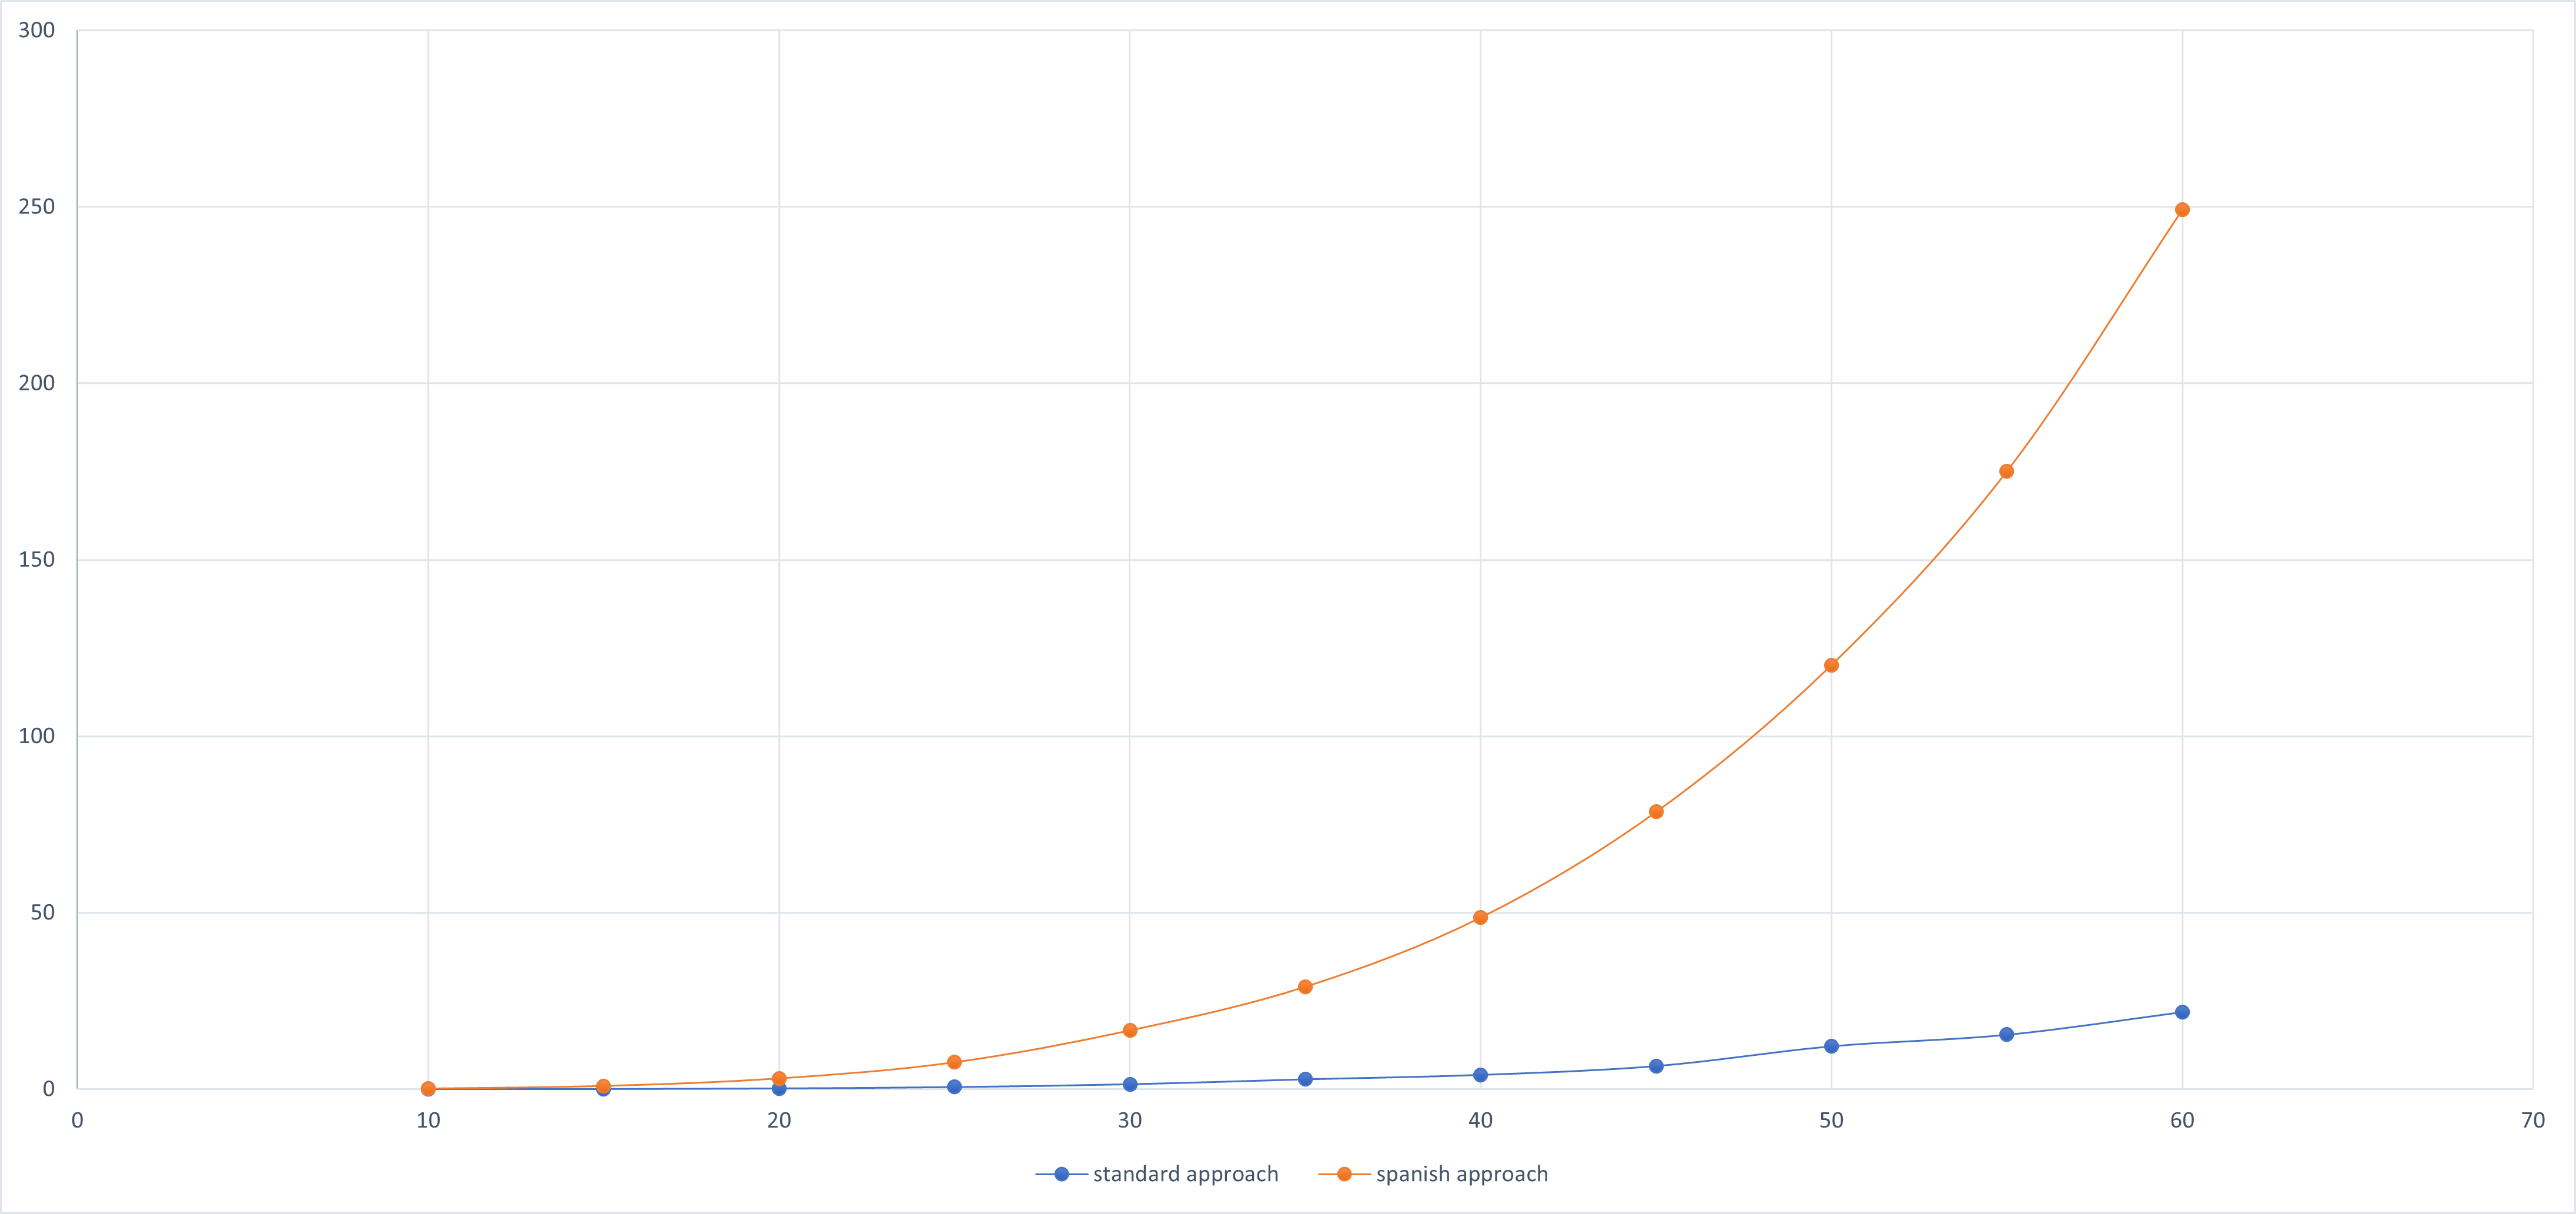
\includegraphics{images/benchmark.png}
\end{figure}

\subsection{דיון לגבי משחק על גרף}
כאשר תיארנו את המשחק על גרף אתכן 
והסיבות לקח היו:
\begin{enumerate}
    \item 
    ככול שמבנה כללי יותר תאוריה שאתה מפתח מתאימה ליותר בעיות.
    \item 
    קיימת תאוריה רחבה שפותחה על גרפים ואתכן שנעזר בה.
    \item 
    מבליט את מהות הבעיה והגדרה הבסיסית ביותר של המשחק.
\end{enumerate}
בפועל כשהצגנו את אלגוריתמים לפתרון המשחק 
התגלתה התמונה המלאה.
שני האלגוריתמים שתיארנו מתארים את המשחק כגרף היות ושני האלגוריתמים בנויים על מטריצת השכנויות.
קשר זה מדגיש ומראה שלפעמים רק תיאור מהות הבעיה מספיק כדי למצוא לבעיה פתרון.

\section{קיום פתרון ומספר הפתרונות עבור משחק על גרף}
עד כה הסתכלנו הצגנו שיטות למציאת פתרון,
שיטות עלו האירו את העובדה
ששאלת קיום הפתרון למשחק על גרף שקולה לשאלת קיום הפתרון למערכת
משוואות לינאריות.
בפרק זה נרצה להוכיח קיום פתרון למשחק לכל גרף.
העובדה שקיים פתרון לכל כל גרף אינה מובנת מעליה.
אחד המקומות ששאלה זה נשאלה היא בספר 
\cite{B3},
בעבודתנו נראה הוכחה קצת שונה בעזרת הכלים שפיתחנו.
אומנם הוכחה קיום פתרון הופיע לראשונה במאמר 
\cite{Sutner}.
כמו כן המחבר כותב שיש רק הוכחה שמבוססת על אלגברה לינארית.

\subsection{הוכחת קיום פתרון על גרף}
\begin{definition}
    תהי 
    $\mathbb{S}$
    קבוצה,
    פעולה בינארית על 
    $\mathbb{S}$
    היא פונקציה
    $\mathbb{S} \times \mathbb{S} \rightarrow \mathbb{S}$
    המתאימה לכל זוג 
    סדור.
    פעולה בינארית 
    עבור הזוג
    $(s_1, s_2)$
    תסומן
    $\langle s_1, s_2 \rangle$.
\end{definition}
\begin{definition}
    מכפלה פנימית 
    היא פעולה
    בינארית
    שמוגדרת לכל זוג וקטורים 
    במרחב וקטורי 
    $\mathbb{S}^n \subseteq \mathbb{R}^n$
    ומעתיקה אותם 
    ל
    $\mathbb{S}$.
    תהי 
    $\mathbb{S}^n \subseteq \mathbb{R}^n$
    מרחב וקטורי עם מכפלה פנימית,
    לכל
    $x,y,z \in \mathbb{S}^n$
    ו
    $\alpha \in \mathbb{S}$,
    פעולה בינארית תקראה מכפלה פנימית אם היא מקיימת
    $4$
    אקסיומות
    הבאות:
    \begin{enumerate}
        \item 
        $\langle x, y \rangle = \langle y,x \rangle$
        \item 
        $\langle x + y, z \rangle = \langle x, z \rangle + \langle y, z \rangle$
        \item 
        $\langle \alpha \ x, y \rangle = \alpha \langle x, y \rangle$
        \item 
        \begin{enumerate}
            \item 
            $\langle x, x \rangle \ge 0$ 
            \item 
            $\langle x, x \rangle = 0 \Longleftrightarrow  x = \vec{0}$ 
        \end{enumerate}
    \end{enumerate}
\end{definition}
\begin{definition}
    \label{def:inner_mul}
    לכל שני וקטורים
    $x, y \in \Zn$
    נגדיר פעולה הבאה:
    \begin{equation}
        x \cdot y = 
        \begin{bmatrix}
            x_1 \\
            x_2 \\
            \cdots \\
            x_n \\
        \end{bmatrix}
        \cdot 
        \begin{bmatrix}
            y_1 \\
            y_2 \\
            \cdots \\
            y_n \\
        \end{bmatrix}
        = 
        x_1 y_1 + x_2 y_2 + \cdots x_n y_n
    \end{equation}
    לפעולה זה
    בין שני וקטורים ב
    $\Zn$
    ניקרא מכפלה סקלרית. 
\end{definition}
\begin{comm}
    \label{comm:not_really_inner_mul}
    פעולה שהגדרנו 
    בהגדרה 
    \ref{def:inner_mul}
    נקראת 
    מכפלה סקלרית
    למרות שהיא
    מקיימת רק 
    $3$
    מתוך 
    $4$
    תכונות של מכפלה סקלרית ב
    -
    $R^n$.   
    תכונה 
    $<\vec{u},\vec{u}> = 0 \Leftrightarrow \vec{u} = \vec{0} $
    לא מתקיימת.
\end{comm}
דוגמה 
שמסבירה את הערה
\ref{comm:not_really_inner_mul}:
\[
    \begin{bmatrix}
    1 \\
    1 \\
    \end{bmatrix}    
    \cdot 
    \begin{bmatrix}
    1 \\
    1 \\
    \end{bmatrix} 
    = 1 + 1 = 0
\]
\begin{comm}
    וקטורים 
    $x, y \in \Zn $
    יקראו מאונכים אחד לשני נסמן זאת 
    $x \perp  y$
    אם המכפלה הסקלרית שהלם שווה 
    ל
    $0$
    $x \cdot y = 0$
\end{comm}
\begin{theorem}
    \label{the: Nul A and Col AT}
    תהי מטריצה 
    $A \in {\mathbb{Z}_2}^{m \times n }$
    אז 
    $\Col A^T \perp \Nul A$
    $\Col A \perp \Nul A^T$
\end{theorem}
\begin{proof}
    תהי 
    מטריצה
    $A \in \mathbb{Z}_2^{m \times n}$
    ניקח 
    $\vec x \in \mathrm{Nul} A$.
    לכן
    $A\vec x=\vec 0$. 
    אז,
    \[
        \vec x \perp \mathrm{Row}A=\mathrm{Col} A^T
    \]
    רצוי לציין 
    שעבור 
    מטריצות 
    $A \in {Z_2}^{m \times n}$
    מאותם שיקולים אותה הוכחה נכונה,
    רק עבור מכפלה הסקלרית שהגדרנו 
    בהגדרה 
    \ref{def:inner_mul}.
\end{proof}
נרצה לחדד תופעה מעניינת שקוראת בשדה וקטורי 
$\Zn$
עם המכפלה הסקלרית שהגדרנו.
עבור השדה הוקטורי 
$\mathbb{R}^n$
לכל מטריצה 
$A \in \mathbb{R}^{m \times n}$
מתקיים 
$\Col A \cap \Nul A^T = \{ \vec{0}\}$.
טענה זה אינה נכונה בשדה 
$\Zn$.
\begin{theorem}
    \label{thrm: clean game has solution}
    לכל משחק על גרף קיים פתרון.
\end{theorem}
\begin{proof}
    כשפיתחנו את 
    שיטת פתרון 
    בעזרת מטריצת השכנויות 
    שהגדרנו
    \ref{def: standard solution},
    הצלחנו לתאר את המשחק בעזרת 
    מערכת משוואות.
    המטריצה שמתארת את המערכת קראנו לה מטריצה שכנויות
    נסמן ב
    $A \in {Z_2}^{n \times n}$.
    נציין כמה עבודות על מטריצת השכנויות:
    \begin{enumerate}
        \item 
        מטריצה סימטרית לפי
        \ref{comm: symetic matrix}
        \item 
        $A$
        המטריצה הינה ריבועית.
        \item 
        האיברים על האלכסון
        מטריצה 
        $A$
        ערכם שווה ל
        $1$.
    \end{enumerate}

    כדי להראות שלמשחק יש פתרון 
    צריך להראות שקיים פתרון למערכת
    \[A \vec{x} = \vec{1} \]
    במקרה ש 
    $A$
    מטריצה הפיכה אז קיים פתרון יחיד.
    עבור המקרה שמטריצה אינה הפיכה 
    כלומר 
    $\Nul A \neq \{ \vec{0}\}$
    ניקח 
    $\vec{x} \in \Nul A$
    מהגדרה מתקיים
    $A\vec{x} = \vec{0}$
    לכן מתקיים:
    \[\vec{x}^T A \vec{x} = \vec{x}^T\vec{0} = 0\]
    נסמן 
    $\vec{x} = [x_1, x_2, \cdots, x_n]^T$
    \begin{align}
        \label{eq: quadratic form}
            \vec{x}^T A \vec{x} &= a_{1,1}x_1^2 + 2(a_{1,2} + a_{2,1})x_1x_2 + \cdots + 2(a_{1,n} + a_{n,1})x_1x_n +  \\
            \nonumber &+ a_{2,2}x_2^2 +  2(a_{2,3} + a_{3,2})x_2x_3 + \cdots  + 2(a_{2,n} + a_{n,2})x_2x_n + \cdots 
    \end{align}
    היות ומטריצה סימטריות
    $a_{i,j} = a_{j,i}$
    לכן
    מתקבל:
    \[a_{i,j} - a_{j,i} = a_{i,j} + a_{j,i} = 1 \]
    נזכיר כי תוצאות של פעולת חיבור וחיסור מודלו 
    $2$
    זהות.
    לכן
    את המשוואה 
    \ref{eq: quadratic form}
    אפשר לפשט:
    \[ \vec{x}^T A \vec{x} = a_{1,1}x_1^2 + a_{2,2} x_2^2 +  a_{n,n} x_n^2\]
    הבחנה נוספת
    לא משנה אם הערך 
    $0$
    או
    $1$
    מתקיים השוויון,
    $x^2 = x$
    לכן פישוט נוסף למשוואה 
    \ref{eq: quadratic form}:
    \[ \vec{x}^T A \vec{x} = a_{1,1}x_1 + a_{2,2} x_2 +  a_{n,n} x_n\]
    לכן קיבלנו 
    $ \vec{x}^T A \vec{x} = 0$
    ומתקיים:
    \[a_{1,1}x_1 + a_{2,2} x_2 +  a_{n,n} x_n = 0\]
    כלומר 
    $\vec{1} \perp  \vec{x}$
    כאשר 
    $x \in \Nul A$
    לפי משפט 
    \ref{the: Nul A and Col AT}
    מתקבל 
    $\vec{1} \in \Col A^T$
    היות ומטריצה סימטרית 
    $A^T = A$
    לכן
    $\vec{1} \in \Col A$
    והוכחנו שלמערכת
    $A\vec{x} = \vec{1}$
    יש פתרון.
\end{proof}
הוכחת קיום הפתרון עבור המשחק כפי שהגדרנו  על גרף הושגה, מסקנה נאיבית שניתן אולי לחשוב היא שלכל מצב התחלתי
אפשרי היה ניתן לפתור את המשחק. בחלק זה של הפרק ננסה לחדד ולהעביר.
\begin{definition}
    \label{def:diff-game}
    משחק אחר שאפשר להציע הוא משחק האורות כללי יותר מוגדר כך:
    לוח הבקרה נשאר זהה למשחק המקורי כלומר, שינוי נורות 
    לאחר לחיצה מתנהג נשאר כפי שהוגדר במשחק המקורי.
    הבדל בין משחק החדש למקורי 
    מצב התחלתי שחלק מנורות דולקות וחלק כבויות ורוצים להגיע למצב סופי שגם בו חלק מנורות דולקות וחלק כבויות.
\end{definition}
עבור המשחק שהגדרנו 
\ref{def:diff-game}
אותו קורא נאיבי יכול להניח שגם עבור משחק שכזה תמיד קיים פתרון.
אם חושבים קצת לעומק קל מאד לבנות דוגמה למשחק על לוח, שאין לו פתרון.
דוגמה אפשרית למקרה שכזה היא לקחת משחק על לוח 
$2 \times 1$
בו מצב התחלתי הוא שהנורה השמאלית ביותר דלוקה ונרצה לעבור למצב הסופי בו כל 
הנורות דולקות.
נרצה להראות שבאמת המשחק אינו פתיר וזה קל כי כמות 
הלוחות השונים שניתן להגיע בעזרת לחיצות היא מצומצמת.
אפשר לתאר את כל המצבים האפשריים לפי 
כל צירופים לא סדורים האפשריים של לחיצות אפשריות.
אם נמספר את הלחצנים לפי שיטת המספור שציינו בהערה 
\ref{ comm: indexing board game}.
אז אוסף כל צירופים הלא סדורים 
של אוסף לחיצות אפשריים הם 
\[
    (), (1), (2), (1,2)
\]
\begin{figure}[ht]
    \caption{מצבי הלוחות לאחר לחיצה של צירוף}
    \centering
    \begin{subfigure}{.20\textwidth}
        \caption{
            עבור צירוף
            $()$
        }
        \[
            \begin{bmatrix}
                0 & 1
            \end{bmatrix}
        \]
    \end{subfigure}
    \begin{subfigure}{.20\textwidth}
        \caption{
            עבור צירוף
            $(1)$
        }
        \[
            \begin{bmatrix}
                1 & 0
            \end{bmatrix}
        \]
    \end{subfigure}
    \begin{subfigure}{.20\textwidth}
        \caption{
            עבור צירוף
            $(2)$
        }
        \[
            \begin{bmatrix}
                1 & 0
            \end{bmatrix}
        \]
    \end{subfigure}
    \begin{subfigure}{.20\textwidth}
        \caption{
            עבור צירוף
            $(1, 2)$
        }
        \[
            \begin{bmatrix}
                0 & 1
            \end{bmatrix}
        \]
    \end{subfigure}%
\end{figure}
כדי לבדוק אם קיים פתרון למשחק הכללי שהגדרנו 
בהגדרה 
\ref{def:diff-game}
נוכל להיעזר בהוכחה
\ref{thrm: clean game has solution}.
\begin{theorem}
    למשחק הזה יש פתרון אם ורק אם וקטור הפרש בין מצב סופי ומצב ההתחלתי אורתוגונלי למרחב 
    העמודות של מטריצת השכנויות של המשחק.
\end{theorem}
\begin{proof}
    נגדיר קודם את המשחק החדש אלגברית.
    לפי משוואה 
    \ref{eq: sum change vectors}
    אפשר לנסח אלגברית את המשחק כך.
    תהי 
    $A$
    מטריצת השכנויות 
    $S_0$
    מצב התחלתי של המשחק 
    ו
    $S_e$
    מצב הסופי של המשחק,
    נחפש צירוף 
    לא סדור של לחיצות 
    $\vec x$
    כך שמתקיים:
    \[
        S_0 + Ax = S_e
    \]
    נעביר אגפים ונקבל:
    \[
         Ax = S_e - S_0
    \]
    אם נחזור ונסתכל על הוכחה
    של משפט 
    \ref{thrm: clean game has solution}
    כל הוכחה בנויה על להוכיח שמצב הסופי 
    שבמקרה של המשחק המקורי הוא 
    $\vec 1$
    שייך ל
    $\Col A$.
    הראינו בהוכחה דרך 
    קלה יותר לבדוק את את זה והיא
    להראות שהוא שמצב
    הסופי 
    שייך 
    $\Nul A$.
    לכן כדי להוכיח שמשחק הכללי כפי שהגדרנו 
    בהגדרה 
    \ref{def:diff-game}
    פתיר, 
    מספיק להראות 
    $S_e - s_0 \in \Nul A$
\end{proof}
\begin{comm}
    דרך קלה לבדוק שוקטור 
    $\vec v \in \mathbb{R}^{n}$
    שייך 
    ל
    $\Nul A$
    של מטריצה 
    $A \in \mathbb{R}^{m \times n}$
    היא לוודא שמתקיים:
    \[ A \vec v = \vec 0\]
\end{comm}
\subsection{מספר הפתרונות עבור כל גרף}
הוכחנו שלכל משחק על גרף שמתחל עם כל לחצנים במצב 
$0$
יש פתרון ניזכר שסדר לחיצות
אינו משנה את התוצאה על הלוח לכן אם נילחץ על הלחצנים בסדר כלשהו 
לפי פתרון נקבל גרף כולו דלוק.

השאלה  שנשאל בפרק זה מה אפשר לומר על מספר פתרונות מפיתוח שעשינו.
נציין קודם שניקרא לשני פתרונות שונים אם קיים לפחות לחצן אחד שמבדיל בין הפתרונות 
כלומר קיים לחצן ששייך לפתרון ראשון ולא שייך לפתרון שני כפי שציינו קודם סדר
לחיצות לא משנה את הפתרון.
לכן פתרון הינו קבוצה של לחצנים.
בנוסף נזכר לפי הערה
\ref{comm: press is uneven presses}
מספר אי זוגי של לחיצות נחשב ללחיצה לכן מספר הלחיצות על אותו לחצן לא משנה 
אלה רק זוגיות של מספר לחיצות 
לכן לכל לחצן יש רק שני מצבים שיכול להיות 
לחוץ 
או לא.
כרגע נראה שקיים כמה פתרונות לדוגמא 
איור
\ref{fig: clic 3 node graph game}
המתאר משחק על גרף בו הצמתים כבויים.
היות וגרף הינו קליקה לכן לחיצה בודדת על אחד הצמתים תדליק את כל הלחצנים.

קבלנו 
$G = \{\{v_1\}, \{v_2\}, \{v_3\} \}$
היא קבוצת של פתרונות.
כלומר כבר הראינו שיש מקרים בהם יש יותר מפתרון אחד.
\begin{figure}[ht]
    \caption{משחק על גרף}
    \label{fig: clic 3 node graph game} 
    % \unsethebrew
    \centering
    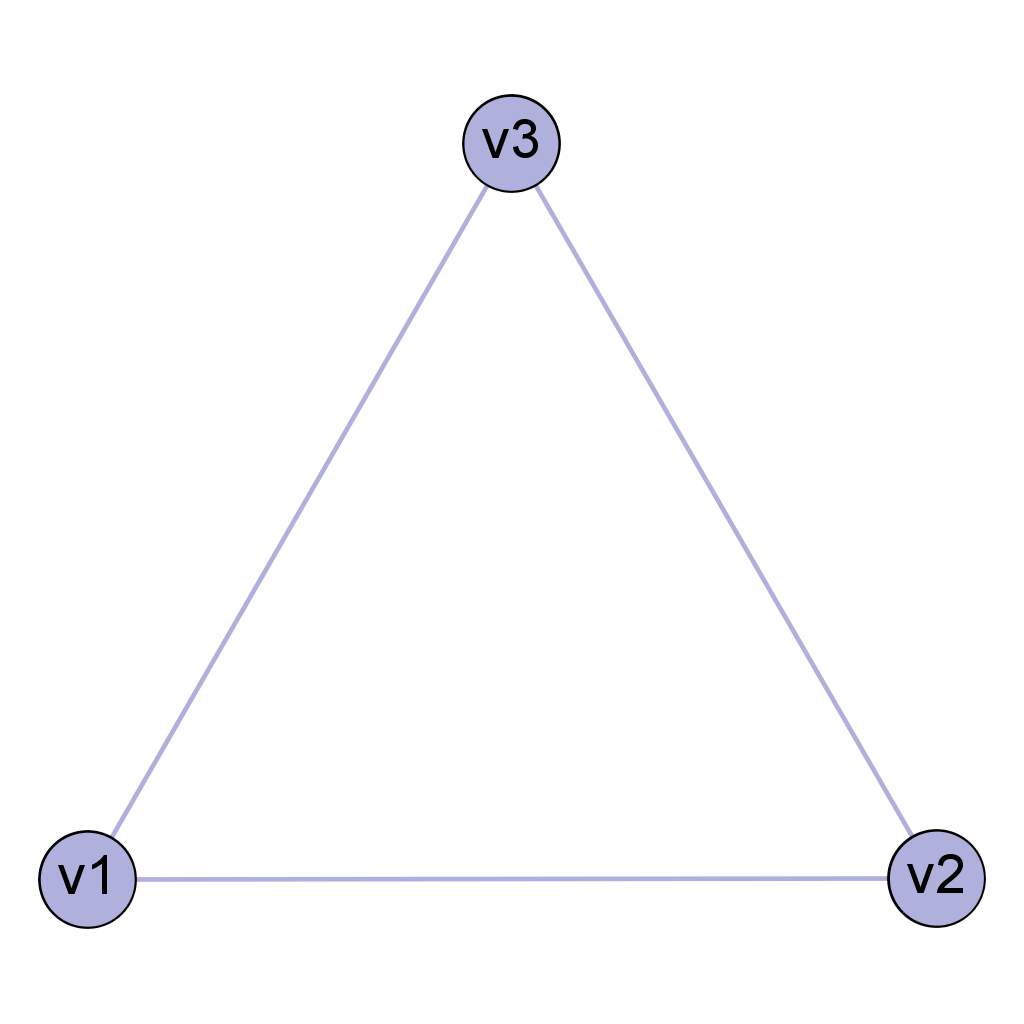
\includegraphics[width=.3\textwidth,keepaspectratio]{images/clic_graph_3_node.png}
\end{figure}

שאלה טביעת שנובעת שנשאלת היא כמה פתרונות יש למשחק מסוים.
כדי לענות על שאלה נצטרך להציג כמה מושגים מאלגברה לינארית.
בשיטת דירוג של גאוס אם ניזכר בקצרה בשיטה ,
אנחנו עוברים שורה שורה ומנסים בעזרת פעולות של שורות 
ליצור עמודות בהם מופיע איבר בודד ששונה מאפס.
\begin{definition}
    איבר מוביל בשורה הוא האביר הראשון בשורה ששונה מאפס 
    לאחר דירוג.
\end{definition}
\begin{definition}
    נעלמים שאברהם מובילים אחרי דירוג אקראו נעלמים מובילים.
\end{definition}
\begin{definition}
    במטריצה מדורגת בשיטת גאוס עבור עמודות שאין בהם איבר מוביל 
    תיקרא עמודה חופשית.
\end{definition}
\begin{definition}
    נעלמים שעמודה שלהם חופשית אחרי דירוג יקראו נעלמים חופשים.
\end{definition}
\begin{definition}
    מספר נעלמים חופשיים במטריצה נקרא
    דרגת החופש.
\end{definition}
ניתן דוגמה קטנה שתסכם את המושגים שהצגנו,
ניקח מטריצה  המדורגת הבאה:
\[
    A = \begin{bmatrix}
        {\color{blue}1} & 0 &  {\color{violet}0} & 0 &  {\color{violet}0} &  {\color{violet}0}\\
        0 &{\color{blue}1} & {\color{violet}0} & 0  &  {\color{violet}0} &  {\color{violet}0}\\
        0 & 0 &  {\color{violet}0} &{\color{blue}1} &  {\color{violet}0} &  {\color{violet}0}
    \end{bmatrix}
\]
בדוגמה צבענו בכחול את האיברים המובילים
ובסגול את עמודות החופשיות.
עבור הדוגמה דרגת החופש היא 3
\begin{comm}
    דרך קלה לחשב את דרגת החופש
    $F(A)$
    של מטריצה 
    $A \in\mathbb{R}^{m \times n}$
    כשידוע שדרגה של מטריצה
    $A$
    הוא 
    $\mathrm{rank}(A) $
    בעזרת הנוסחה הבאה:
    \[
        F(A) = n - rank(A)
    \]
\end{comm}
לאחר שהגדרנו את מושג דרגת החופש נוכל לנסח את המפשט המרכזי של הפרק.
\begin{theorem}
    מספר הפתרונות של משחק 
    שווה ל 
    $2^{k}$
    כאשר 
    $k$
    שווה לדרגת החופש של מטריצה
    $A$
    של פתרון הסטנדרטי
\end{theorem}
היות לכל משחק ניתן להגיר מטריצת שכנויות של משחק שהגדרנו 
ב
\ref{def: neighbor matrix}
ופתרונות של משחק וקטורים
$X$
של מערכת
$A \vec x = \vec{1}$
כאשר 
$A$
מטריצת שכנויות.
ידוע שקיים פתרון למשחק ואם הוא משחק שמתחיל שמצב כל הנורות הוא
$0$
אז יש משפט 
\ref{thrm: clean game has solution}.
שמוכיח שקיים פתרון.

היות ומניחים שיש כמה פתרונות אפשר לתאר את כל פתרונות כ
$x = x_n + x_0$
כאשר 
$x_n \in \Nul(A)$ ,
$x_0$ 
פתרון פרטי שידוע שקיים 
ו
$x$
כל פתרונות הכללים.

לכן מספר פתרונות כללים שווה למספר פתרונות במרחב האפס.
ידוע שמספר פתרונות במרחב האפס תלוי לדרגת החופש ולכן מספר הווקטורים שפורשים
את מרחב האפס שווה לדרגת החופש שנסמן ב
$k$.
כמות הווקטורים במרחב זה שווה לכל וקטורים שניתן ליצור בצירוף לינארי 
\[x = a_1 x_1 + a_1 x_1 + a_2 x_2 + \cdots + a_k x_k\]
כאשר הערכים של
$a_i \in Z_2$
לכן 
לכל מקדם יכול להיות
$2$
ערכים,
לכן כל הקונבנציות האפשריות 
$2^k$
ששווה
לכמות הווקטורים 
במרחב האפס וכמות הפתרונות השונים של המשחק.

הבחנה נוספת ומעניינת שנרצה לציין היא בנושא חסם עליון לכמות הפתרונות.
חסם עליון טריוויאלי לכמות המקסימלית של פתרונות היא 
$2^n$
פתרונות כאשר
$n$
שווה למספר הלחצנים כלומר לא יכול להיות יותר פתרונות מאשר כמות הלחיצות השונות האפשריות במשחק.
\begin{comm}
    עבור משחק לוח מלבני
    בגודל 
    $m \times n$
    קיים לכל יותר 
    $2^k$
    כאשר 
    $k = \min\{m,n\}$
    פתרונות שונים
\end{comm}
הערה זה נכונה לפי גישה פתרון הספרדית
שהגדרנו
\ref{def: spanish way}
ניתן לתרגם את משחק ל
$k$
משוואות 
ש
$k$
יכול להיות מספר שורות או עמודות 
לכן ניקח את המספר הקטן יותר.

לסיכום נרצה להציג טבלה של מספר הפתרונות כתלות לממדי הלוח.
את הטבלה אפשר לראות באיור 
\ref{fig:num-sol-in-table}
כאשר, השורות ועמודות בטבלה מייצגות 
את ממדי הלוח בהתאמה.

\begin{figure}
    \caption{טבלה מתארת מספר פתרונות בלוחות 
    $m \times n$
    }
    \centering
    \label{fig:num-sol-in-table}
    \begin{english}
        \begin{tabular}{ |c||c|c|c|c|c|c|c|c|c| }
            \hline
            \ & 1 & 2 & 3 & 4 & 5 & 6 & 7 & 8 & 9 \\
            \hline
            \hline
            1 & 1 & 2 & 1 & 1 & 2 & 1 & 1 & 2 & 1 \\
            \hline
            2 & 2 & 1 & 4 & 1 & 2 & 1 & 4 & 1 & 2 \\
            \hline
            3 & 1 & 4 & 1 & 1 & 8 & 1 & 1 & 4 & 1 \\
            \hline
            4 & 1 & 1 & 1 & 16 & 1 & 1 & 1 & 1 & 16 \\
            \hline
            5 & 2 & 2 & 8 & 1 & 4 & 1 & 16 & 2 & 2 \\
            \hline
            6 & 1 & 1 & 1 & 1 & 1 & 1 & 1 & 64 & 1 \\
            \hline
            7 & 1 & 4 & 1 & 1 & 16 & 1 & 1 & 4 & 1 \\
            \hline
            8 & 2 & 1 & 4 & 1 & 2 & 64 & 4 & 1 & 2 \\
            \hline
            9 & 1 & 2 & 1 & 16 & 2 & 1 & 1 & 2 & 256 \\
            \hline
        \end{tabular}
    \end{english}
\end{figure}

\section{פתרון אופטימלי עבור לוחות מלבניים}
בפרק זה נציג סוג מסוים של פתרונות,
סוג זה אקרה פתרון אופטימלי.
סוג זה של פתרון מקל רבות על המשחק 
כיוון שמצמצם את כמות הלחיצות האפשריות בכל מצב במשחק.
\begin{definition}
    \label{def: opt-sol}
    פתרון אופטימלי של משחק הינו פתרון 
    בו שינוי מצב כל הנורות 
    היה יחיד.
    כלומר 
    השחקן פתר את המשחק כאשר 
    כל נורה עברו ממצב התחלתי למצב הסופי פעם אחת בלבד
\end{definition}
באיור 
\ref{fig: min sol 2x3}
ניתן דוגמא לפתרון מינמלי 
בלוח 
$2 \times 3$.
כשלוחצים על לחצנים 
$3, 4$
על לוח כל נורות נדלקות ואף 
אחת מהם לא נכבה באף שלב של לחיצה.

\begin{figure}[ht]
    \caption{פתרון מינמלי של משחק}
    \label{fig: min sol 2x3}
    % \unsethebrew
    \centering
    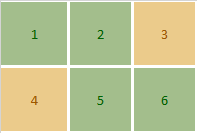
\includegraphics[width=.3\textwidth,keepaspectratio]{images/min_sol_2x3.PNG}
\end{figure}

נרצה לחדד ולהדגיש עד כמה קל למצוא פתרונות אופטימלי.
אם ניקח לוח 
$2 \times 3$
כפי שמתואר 
באיור 
\ref{fig: min sol 2x3},
ונתבונן במספר כל הפתרונות שיש ללוח זה
כפי
שמתואר בטבלה 
\ref{fig:num-sol-in-table}
ניראה שיש 
$4$
פתרונות.
קיימים שני פתרונות אופטימליים 
ושני פתרונות לא אופטימליים,
ופה נשאלת השאלה כמה פתרונות בהתבוננות חפזה הקרואה רואה.
כנראה ששני הפתרונות האופטימליים מיידית נמצאו. כנראה גם שכדי למצוא פתרונות הנותרים 
נצטרך לקחת דף ועט ולחפש אותם גם עבור לוח בממד מצומצם שכזה.
את כל ארבעת הפתרונות נציג באיור 
\ref{fig:all-2x3-sol}.

\begin{figure}[ht]
    \caption{משחק על גרף לדוגמה}
    \label{fig:all-2x3-sol}
    \centering
    \begin{subfigure}{.20\textwidth}
        % \unsethebrew
        \centering
        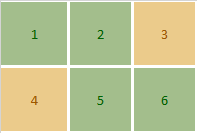
\includegraphics{images/min_sol_2x3.PNG}
        % \sethebrew
    \end{subfigure}%
    \begin{subfigure}{.20\textwidth}
        % \unsethebrew
        \centering
        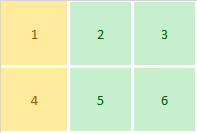
\includegraphics{images/2x3_2.png}
        % \sethebrew
    \end{subfigure}%
    \begin{subfigure}{.20\textwidth}
        % \unsethebrew
        \centering
        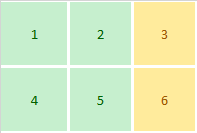
\includegraphics{images/2x3_3.png}
        % \sethebrew
    \end{subfigure}%
    \begin{subfigure}{.20\textwidth}
        % \unsethebrew
        \centering
        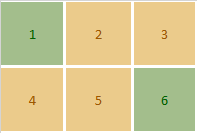
\includegraphics{images/2x3_4.png}
        % \sethebrew
    \end{subfigure}%
\end{figure}

השאלה שנפתור בפרק זה לאיזה לוחות קיים פתרון מינמלי כאשר מצב התחלתי הוא שכל הנורות במצב
$0$.

\subsection{הוכחת אי קיום לפתרון אופטימלי על לוחות ששני הממדים גדולים מ
\texorpdfstring{$4 \times 4$}{4 x 4}}
לפני שבאמת נוכיח את הטענה 
נציין את משמעות ששני הממדים גדולים מ
$4 \times 4$.
\begin{comm}
    \label{comm:sol to 2 x m}
    קיים פתרון אופטימלי למשחק 
    $2 \times m$
    כאשר 
    $m$
    הוא אי זוגי.
\end{comm}
הפתרון הוא פשוט נלחץ פעם אחת בשורה ראשונה ופעם אחרת בשורה השנייה כמו שמתואר באיור 
\ref{fig: 2x9 have min sol}.

\begin{figure}[ht]
    \caption{פתרון ללוח 
    $2 \times 9$}
    \label{fig: 2x9 have min sol}
    % \unsethebrew
    \centering
    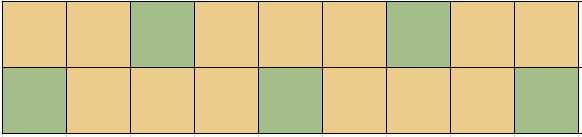
\includegraphics[width=.5\textwidth,keepaspectratio]{images/2xm_sol.PNG}
\end{figure}

הסיבה שקיים פתרון אופטימלי לכל לוח 
$2 \times m$
שפשוט שיטת הפתרון שהצגנו ניתן להרחבה לכל 
$m$.
ניקח לדוגמה את איור 
\ref{fig: 2x9 have min sol}
אם נוסיף שתי עמודות ימינה 
אז לחיצה על שורה העליונה 
בעמודה הימנית ביותר תפתור את המשחק.

בגלל הערה 
\ref{comm:sol to 2 x m}
הגבלנו חיפוש לפתרון אופטימלי ללוחות 
ששני הממדים שלהם גדולים מ
$4 \times 4$.
בכך פסלנו את אינסוף הלוחות שתיארנו בהערה 
\ref{comm:sol to 2 x m}.

כדי להוכיח טענת הפרק נעזר בלוח שמתואר כך,
ללוח יש משבצת שהיא ראשית הצירים 
נסמן אותה כ 
$a_{1,1}$.
בלוח זה  הצירים ממשיכים אינסוף ימינה ולמעלה.
נתאר את המשחק הנתון בעזרת מטריצה אינסופית.
\begin{theorem}
    \label{thm:cant-press-a11}
    אין אף פתרון 
    אופטימלי בו המשבצת בראשית הצירים נלחצה 
\end{theorem}
\begin{proof}
    לאחר לחיצה על 
    $a_{1,1}$
    מתקבל הלוח הבאה:
    \[
        \begin{bmatrix}
            1 & 1 & 0 & 0 \\
            1 & 0 & 0 & 0 \\
            0 & 0 & 0 & 0 \\
        \end{bmatrix}
    \]
    כדי להדליק 
    את הנורה
    $a_{2,2}$
    נצטרך 
    ללחוץ
    $a_{2,3}$
    או 
    $a_{3,2}$
    .
    אם נילחץ על
   $a_{2,3}$
   נקבל את הלוח הבאה:
   \[
        \begin{bmatrix}
            1 & 1 & 1 & 0 \\
            1 & 1 & 1 & 1 \\
            0 & 0 & 1 & 0 \\
        \end{bmatrix}
    \]
    נשים לב כי הגענו למבוי סתום כי
    ניתן להדליק את 
    $a_{3,2}$
    רק על ידי לחיצה על 
   $a_{4,2}$ 
   ואז לא היה ניתן להדליק את 
   $a_{3,1}$.
   ניתוח דומה אפשר לתאר עבור 
   לחיצה על 
   $a_{3,2}$.
\end{proof}
לפי טענה
\ref{thm:cant-press-a11}
אם ברצוננו למצוא למשחק האינסופי שהגדרנו פתרון מינמלי לא נוכל 
להדליק את נורה 
$a_{1,1}$
על ידי לחיצה עליו.
לכן על מנת להדליק את 
$a_{1,1}$
נלחץ על 
$a_{1,2}$.
\begin{theorem}
    \label{thm:cant-press-a12}
    אין אף פתרון 
    אופטימלי בו נלחצה 
    משבצת
    $a_{1,2}$
\end{theorem}
\begin{proof}
    כדומה להוכחה 
    טענה 
    \ref{thm:cant-press-a11}
    נגיע למצב סתום.
    אם נסתכל על מצב הלוח לאחר לחיצה על משבצת 
   $a_{1,2}$ 
   ניראה כי יש סידרת לחיצות מאולצת כדי להדליק נורות מסוימות.
   \[
        \begin{bmatrix}
            1 & 1 & 1 & 0 & 0 \\
            0 & 1 & 0 & 0 & 0 \\
            0 & 0 & 0 & 0 & 0 \\
            0 & 0 & 0 & 0 & 0 \\
            0 & 0 & 0 & 0 & 0 \\
            0 & 0 & 0 & 0 & 0
        \end{bmatrix}
    \]
    כדי להדליק את הנורות 
    $a_{2,1}$
    נהיה חייבים ללחוץ על 
    $a_{3,1}$.
    כדי להדליק את הנורות 
    $a_{2,3}$
    נהיה חייבים ללחוץ על 
    $a_{2,4}$.
    כדי להדליק את הנורות 
    $a_{3,3}$
    נהיה חייבים ללחוץ על 
    $a_{4,3}$.
    כדי להדליק את הנורות 
    $a_{5,2}$
    נהיה חייבים ללחוץ על 
    $a_{6,2}$.
    כדי להדגיש את הכפתורים שנלחצו נסמן
    אותם 
    $*$
    ונקבל את הלוח הבאה:
    \[
        \begin{bmatrix}
            1 & * & 1 & 1 & 0 \\
            1 & 1 & 1 & * & 1 \\
            * & 1 & 1 & 1 & 0 \\
            1 & 1 & * & 1 & 0 \\
            0 & 1 & 1 & 0 & 0 \\
            1 & * & 1 & 0 & 0
        \end{bmatrix}
    \]
    נשים לב ששוב הגענו למבוי סתום.
\end{proof}
אפשר להחליף בין הצירים ולקבל בעזרת אותה הוכחה 
למה לא קיים פתרון 
בו נלחצת משבצת 
$a_{2,1}$.
היות ועברנו על כל האפשרויות שאפשר 
לנסות להדליק את 
$a_{1,1}$
והראינו שבכל מצב מגיעים למבוי סתום.
\begin{corollary}
    למשחק אינסופי שכזה לא קיים פתרון אופטימלי.
\end{corollary}
\begin{corollary}
    למשחק 
    $ n \times 4$
    לא קיים פתרון אופטימלי
    כאשר 
    $n > 4$
\end{corollary}
עבור משחק שכזה
אותם 
טענות
\ref{thm:cant-press-a11}
ו
\ref{thm:cant-press-a12}
מתקיימות.
עבור 
תחילת משחק 
מלחיצה על 
$a_{2,1}$
נקבל את סידרת לחיצות המאולצת
$\{a_{2,1}, a_{1,3}, a_{3,4}, a_{4,2}, a_{6,3}\}$
שמתוארת בלוח הבאה:
\[
    \begin{bmatrix}
        1 & 1 & * & 1\\
        * & 1 & 1 & 1\\
        1 & 1 & 1 & *\\
        1 & * & 1 & 1\\
        0 & 1 & 1 & 0\\
        0 & 1 & * & 1
    \end{bmatrix}
\]
והגענו שוב למבוי סתום.
\begin{corollary}
    \label{thrm: bigger then 7x7 board no minimal solution}
    במשחק על לוח 
    $m \times n$
    שמתקיים
    $\min(m,n) > 4$
    למשחק אין פתרון אופטימלי
\end{corollary}

\subsection{אלגוריתם למציאת פתרון אופטימלי}
קיימים מספר דרכים למציאת פתרון אופטימלי.
אפשר לנסות ולחפש פתרון ידנית.
דרך נוספת היא לעבור על כל הפתרונות של משחק רגיל ולבדוק עם יש מבניהם פתרון 
אופטימלי.
נציעה דרך אחרת לחפש פתרון 
מינמלי
והיא בעזרת להשתמש באותה מטריצה שכנויות כפי שהגדרנו רק להגדיר 
את זה שהיא על חוג 
$\mathbb{Z}$.
בעזרת שימוש בחוג 
$\mathbb{Z}$
מאלצים את שפתרונות המתקבלים
שידליקו כל נורות אך ורק פעם אחת,
זאת מתקיים בעקבות 
משוואות האילוצים שהגדרנו ב
\ref{ def: depndeciy equation}
שמאלצות את הסכום להיות שווה לאחד
,
אם נסתכל על נוסחה של משוואת האילוצים הכללים 
נוסחה
\ref{eq: depndeciy equation}
היות וחיבור על השלמים לכן 
מאולצים במשוואה זה שהיה לחצן בודד לחוץ 
לכן פתרון מערכת המשוואות מתאר פתרון 
מינמלי של משחק.
התיאוריה שפיתחנו באלגברה לינארית הייתה תקפה לשדות 
אבל כלי תכנות שהשתמשנו
בעבודה זה יודע לפתור גם על חוג של השלמים 
והסמכנו על הכלי כדי לבדוק את המקרים
שממדים שייכם לקבוצה 
$\{ (m,n) : 2 < m,n <7 \}$
וקיבלנו שהלוח
היחיד בקבוצת הממדים העלו שיש לו פתרון מינמלי 
הוא
לוח 
$4 \times 4$
ופתרון מתואר באיור 
\ref{fig:4x4_have_min_sol}.

\begin{figure}[ht]
    \caption{פתרון ללוח 
    $4 \times 4$}
    \label{fig:4x4_have_min_sol}
    % \unsethebrew
    \centering
    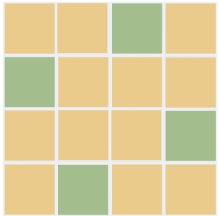
\includegraphics[width=.3\textwidth,keepaspectratio]{images/4x4_sol.PNG}
\end{figure}

\newpage
\section{נספחים}
מימוש של הפרויקט בוצע על ידי 
שפת תוכנה 
{Python}
בעזרת הכלי
{Sage}
וספריות מתמטיות נוספות.
\hypertarget{generate-matrix}{%
\subsection{יצירת מטריצת שכנויות}\label{generate-matrix}}
קוד זה יוצר מטריצת שכנויות של משחק על לוח 
$m \times n$.
\begin{english}
    \begin{tcolorbox}[breakable, size=fbox, boxrule=1pt, pad at break*=1mm,colback=cellbackground, colframe=cellborder]
\prompt{In}{incolor}{8}{\boxspacing}
\begin{Verbatim}[commandchars=\\\{\}]
\PY{k+kn}{import} \PY{n+nn}{numpy} \PY{k}{as} \PY{n+nn}{np}
\PY{c+c1}{\PYZsh{} to prove the minimal case on not square we need to build matrix for not rectangler board}
\PY{k}{def} \PY{n+nf}{genenerate\PYZus{}neighbord\PYZus{}matrix\PYZus{}m\PYZus{}n}\PY{p}{(}\PY{n}{m}\PY{p}{,}\PY{n}{n}\PY{p}{)} \PY{o}{\PYZhy{}}\PY{o}{\PYZgt{}} \PY{n}{np}\PY{o}{.}\PY{n}{array}\PY{p}{:}
    \PY{n}{mat} \PY{o}{=} \PY{n}{np}\PY{o}{.}\PY{n}{zeros}\PY{p}{(}\PY{p}{(}\PY{n}{m}\PY{o}{*}\PY{n}{n}\PY{p}{,} \PY{n}{m}\PY{o}{*}\PY{n}{n}\PY{p}{)}\PY{p}{,} \PY{n}{dtype}\PY{o}{=} \PY{n}{np}\PY{o}{.}\PY{n}{int8}\PY{p}{)}

    \PY{c+c1}{\PYZsh{} the general case}
    \PY{k}{for} \PY{n}{j} \PY{o+ow}{in} \PY{n+nb}{range}\PY{p}{(}\PY{l+m+mi}{0}\PY{p}{,} \PY{n}{m}\PY{o}{*}\PY{n}{n}\PY{p}{)}\PY{p}{:}
        \PY{k}{if} \PY{n}{j}\PY{o}{\PYZhy{}}\PY{n}{n} \PY{o}{\PYZgt{}} \PY{o}{\PYZhy{}}\PY{l+m+mi}{1} \PY{p}{:}
            \PY{n}{mat}\PY{p}{[}\PY{n}{j}\PY{o}{\PYZhy{}}\PY{n}{n}\PY{p}{,}\PY{n}{j}\PY{p}{]} \PY{o}{=} \PY{l+m+mi}{1}

        \PY{k}{if} \PY{n}{j} \PY{o}{\PYZpc{}} \PY{n}{n} \PY{o}{!=} \PY{l+m+mi}{0} \PY{p}{:}
            \PY{n}{mat}\PY{p}{[}\PY{n}{j}\PY{o}{\PYZhy{}}\PY{l+m+mi}{1}\PY{p}{,}\PY{n}{j}\PY{p}{]} \PY{o}{=} \PY{l+m+mi}{1}

        \PY{n}{mat}\PY{p}{[}\PY{n}{j}\PY{p}{,}\PY{n}{j}\PY{p}{]} \PY{o}{=} \PY{l+m+mi}{1}

        \PY{k}{if} \PY{p}{(}\PY{n}{j}\PY{o}{+}\PY{l+m+mi}{1}\PY{p}{)} \PY{o}{\PYZpc{}} \PY{n}{n} \PY{o}{!=} \PY{l+m+mi}{0} \PY{p}{:}
            \PY{n}{mat}\PY{p}{[}\PY{n}{j}\PY{o}{+}\PY{l+m+mi}{1}\PY{p}{,}\PY{n}{j}\PY{p}{]} \PY{o}{=} \PY{l+m+mi}{1}

        \PY{k}{if} \PY{n}{j}\PY{o}{+}\PY{n}{n} \PY{o}{\PYZlt{}} \PY{n}{m}\PY{o}{*}\PY{n}{n} \PY{p}{:}
            \PY{n}{mat}\PY{p}{[}\PY{n}{j}\PY{o}{+}\PY{n}{n}\PY{p}{,}\PY{n}{j}\PY{p}{]} \PY{o}{=} \PY{l+m+mi}{1}
    
    \PY{k}{return} \PY{n}{mat}
\PY{k}{def} \PY{n+nf}{genenerate\PYZus{}neighbord\PYZus{}matrix}\PY{p}{(}\PY{n}{n}\PY{p}{)} \PY{o}{\PYZhy{}}\PY{o}{\PYZgt{}} \PY{n}{np}\PY{o}{.}\PY{n}{array}\PY{p}{:}   
    \PY{k}{return} \PY{n}{genenerate\PYZus{}neighbord\PYZus{}matrix\PYZus{}m\PYZus{}n}\PY{p}{(}\PY{n}{n}\PY{p}{,}\PY{n}{n}\PY{p}{)}

\PY{n+nb}{print}\PY{p}{(}\PY{l+s+s1}{\PYZsq{}}\PY{l+s+s1}{Adj matrix for 3,2 board:}\PY{l+s+s1}{\PYZsq{}}\PY{p}{)}
\PY{n+nb}{print}\PY{p}{(}\PY{n}{genenerate\PYZus{}neighbord\PYZus{}matrix\PYZus{}m\PYZus{}n}\PY{p}{(}\PY{l+m+mi}{3}\PY{p}{,}\PY{l+m+mi}{2}\PY{p}{)}\PY{p}{)}
\end{Verbatim}
\end{tcolorbox}
    \begin{Verbatim}[commandchars=\\\{\}]
Adj matrix for 3,2 board:
[[1 1 1 0 0 0]
 [1 1 0 1 0 0]
 [1 0 1 1 1 0]
 [0 1 1 1 0 1]
 [0 0 1 0 1 1]
 [0 0 0 1 1 1]]
    \end{Verbatim}
\end{english}

    \newpage
    \hypertarget{solver-based-on-adjacency-matrix}{%
\subsection{מציאת פתרון}\label{solver-based-on-adjacency-matrix}}
מתאר אלגוריתם למציאת פתרון בעזרת ממטריצת השכנויות.
הפתרון המתקבל הם וקטורי עמודות.
ניקח לדוגמה את הפתרון
$(1, 0, 1, 0, 1, 0, 1, 0, 1^)$
עבור לוח 
$3 \times 3$
את אותו פתרון נתאר בעזרת מטריצה כך:
\[
    \begin{bmatrix}
        1 & 0 & 1 \\
        0 & 1 & 0 \\
        1 & 0 & 1
    \end{bmatrix}
\]
\begin{english}
    \begin{tcolorbox}[breakable, size=fbox, boxrule=1pt, pad at break*=1mm,colback=cellbackground, colframe=cellborder]
\prompt{In}{incolor}{7}{\boxspacing}
\begin{Verbatim}[commandchars=\\\{\}]
\PY{k+kn}{from} \PY{n+nn}{sage}\PY{n+nn}{.}\PY{n+nn}{all} \PY{k+kn}{import} \PY{o}{*}
\PY{n}{n} \PY{o}{=} \PY{l+m+mi}{3}
\PY{n}{A} \PY{o}{=} \PY{n}{Matrix}\PY{p}{(}\PY{n}{Integers}\PY{p}{(}\PY{l+m+mi}{2}\PY{p}{)}\PY{p}{,}\PY{n}{genenerate\PYZus{}neighbord\PYZus{}matrix}\PY{p}{(}\PY{n}{n}\PY{p}{)}\PY{p}{)} \PY{c+c1}{\PYZsh{} A = adjacency matrix}
\PY{n}{Y} \PY{o}{=} \PY{n}{vector}\PY{p}{(}\PY{p}{[}\PY{l+m+mi}{1} \PY{k}{for} \PY{n}{x} \PY{o+ow}{in} \PY{n+nb}{range}\PY{p}{(}\PY{n}{n}\PY{o}{*}\PY{o}{*}\PY{l+m+mi}{2}\PY{p}{)}\PY{p}{]}\PY{p}{)} \PY{c+c1}{\PYZsh{} Y = ( 1, 1, ..., 1)}
\PY{n}{X} \PY{o}{=} \PY{n}{A}\PY{o}{.}\PY{n}{solve\PYZus{}right}\PY{p}{(}\PY{n}{Y}\PY{p}{)}
\PY{n+nb}{print}\PY{p}{(}\PY{l+s+s1}{\PYZsq{}}\PY{l+s+s1}{Solution for 3x3 board:}\PY{l+s+s1}{\PYZsq{}}\PY{p}{)}
\PY{n+nb}{print}\PY{p}{(}\PY{n}{X}\PY{p}{)}
\end{Verbatim}
\end{tcolorbox}

    \begin{Verbatim}[commandchars=\\\{\}]
Solution for 3x3 board:
(1, 0, 1, 0, 1, 0, 1, 0, 1)
    \end{Verbatim}
\end{english}

    \hypertarget{solver-based-on-calculating-raw-by-raw}{%
\subsection{אלגוריתם מבוסס על מילוי עקבי}\label{solver-based-on-calculating-raw-by-raw}}
שיטת הפתרון השניה שהצגנו בעבודה.
הקוד מחולק לשלושה פונקציות: פעולת דירוג של מטריצה לפי שיטה, פונקציה שפותרת את המערכת 
ופונקציה שעוטפת את שני הפונקציה וממש את השיטה כולה.
הפתרון מוצג כוקטור עמודה כמו שתיארנו ב
\ref{solver-based-on-adjacency-matrix}.
\begin{english}
    \begin{tcolorbox}[breakable, size=fbox, boxrule=1pt, pad at break*=1mm,colback=cellbackground, colframe=cellborder]
\prompt{In}{incolor}{3}{\boxspacing}
\begin{Verbatim}[commandchars=\\\{\}]
\PY{c+c1}{\PYZsh{} row operation on mat to generate the solution for [n, n**2\PYZhy{}1]}
\PY{k}{def} \PY{n+nf}{gaussian\PYZus{}elimination\PYZus{}spanish\PYZus{}alg}\PY{p}{(}\PY{n}{mat} \PY{p}{:} \PY{n}{np}\PY{o}{.}\PY{n}{array}\PY{p}{,} \PY{n}{sol\PYZus{}vec} \PY{p}{:} \PY{n}{np}\PY{o}{.}\PY{n}{array}\PY{p}{)}\PY{p}{:}
    \PY{n}{n} \PY{o}{=} \PY{n+nb}{int}\PY{p}{(}\PY{n}{sqrt}\PY{p}{(}\PY{n}{mat}\PY{o}{.}\PY{n}{shape}\PY{p}{[}\PY{l+m+mi}{0}\PY{p}{]}\PY{p}{)}\PY{p}{)}
    \PY{c+c1}{\PYZsh{}all rows but the last one}
    \PY{k}{for} \PY{n}{i} \PY{o+ow}{in} \PY{n+nb}{range}\PY{p}{(}\PY{l+m+mi}{0}\PY{p}{,} \PY{n}{n}\PY{o}{*}\PY{o}{*}\PY{l+m+mi}{2}\PY{o}{\PYZhy{}}\PY{n}{n}\PY{p}{)}\PY{p}{:}
        \PY{c+c1}{\PYZsh{} the lamp that is affected}
        \PY{n}{affected\PYZus{}lamp} \PY{o}{=} \PY{n}{i} \PY{o}{+} \PY{n}{n}
        \PY{n}{row\PYZus{}i} \PY{o}{=} \PY{n}{mat}\PY{p}{[}\PY{n}{i}\PY{p}{]}\PY{p}{[}\PY{p}{:}\PY{n}{affected\PYZus{}lamp}\PY{o}{+}\PY{l+m+mi}{1}\PY{p}{]}
        \PY{c+c1}{\PYZsh{} check rows below}
        \PY{c+c1}{\PYZsh{} for j in range(i+1, n**2):}
        \PY{k}{for} \PY{n}{j} \PY{o+ow}{in} \PY{p}{[}\PY{n}{i}\PY{o}{\PYZhy{}}\PY{l+m+mi}{1} \PY{o}{+} \PY{n}{n}\PY{p}{,} \PY{n}{i}\PY{o}{+}\PY{n}{n}\PY{p}{,} \PY{n}{i}\PY{o}{+}\PY{n}{n}\PY{o}{+}\PY{l+m+mi}{1}\PY{p}{,} \PY{n}{i}\PY{o}{+} \PY{l+m+mi}{2}\PY{o}{*}\PY{n}{n}\PY{p}{]}\PY{p}{:}
            \PY{k}{if} \PY{n}{j}\PY{o}{\PYZgt{}} \PY{o}{\PYZhy{}}\PY{l+m+mi}{1} \PY{o+ow}{and} \PY{n}{j} \PY{o}{\PYZlt{}} \PY{n}{n}\PY{o}{*}\PY{o}{*}\PY{l+m+mi}{2} \PY{o+ow}{and} \PY{n}{mat}\PY{p}{[}\PY{n}{j}\PY{p}{]}\PY{p}{[}\PY{n}{affected\PYZus{}lamp}\PY{p}{]} \PY{o}{==} \PY{l+m+mi}{1}\PY{p}{:}
                \PY{n}{row\PYZus{}j} \PY{o}{=} \PY{n}{mat}\PY{p}{[}\PY{n}{j}\PY{p}{]}\PY{p}{[}\PY{p}{:}\PY{n}{affected\PYZus{}lamp}\PY{o}{+}\PY{l+m+mi}{1}\PY{p}{]}
                \PY{n}{row\PYZus{}j} \PY{o}{=} \PY{n}{row\PYZus{}j} \PY{o}{+} \PY{n}{row\PYZus{}i}
                \PY{n}{row\PYZus{}j} \PY{o}{=} \PY{n}{row\PYZus{}j} \PY{o}{\PYZpc{}} \PY{l+m+mi}{2}
                \PY{n}{mat}\PY{p}{[}\PY{n}{j}\PY{p}{]}\PY{p}{[}\PY{p}{:}\PY{n}{affected\PYZus{}lamp}\PY{o}{+}\PY{l+m+mi}{1}\PY{p}{]} \PY{o}{=} \PY{n}{row\PYZus{}j}
                \PY{n}{sol\PYZus{}vec}\PY{p}{[}\PY{n}{j}\PY{p}{]} \PY{o}{=} \PY{p}{(} \PY{n}{sol\PYZus{}vec}\PY{p}{[}\PY{n}{j}\PY{p}{]} \PY{o}{+} \PY{n}{sol\PYZus{}vec}\PY{p}{[}\PY{n}{i}\PY{p}{]} \PY{p}{)} \PY{o}{\PYZpc{}} \PY{l+m+mi}{2}

\PY{c+c1}{\PYZsh{} get result to [n, n**2\PYZhy{}1] from solution [0, n\PYZhy{}1]               }
\PY{k}{def} \PY{n+nf}{mul\PYZus{}mat\PYZus{}sol\PYZus{}based\PYZus{}on\PYZus{}res}\PY{p}{(}\PY{n}{mat} \PY{p}{:} \PY{n}{np}\PY{o}{.}\PY{n}{array}\PY{p}{,} \PY{n}{end\PYZus{}state} \PY{p}{:} \PY{n+nb}{list}\PY{p}{,} \PY{n}{res} \PY{p}{:} \PY{n+nb}{list}\PY{p}{)}\PY{p}{:}
    \PY{n}{n} \PY{o}{=} \PY{n+nb}{int}\PY{p}{(}\PY{n}{sqrt}\PY{p}{(}\PY{n}{mat}\PY{o}{.}\PY{n}{shape}\PY{p}{[}\PY{l+m+mi}{0}\PY{p}{]}\PY{p}{)}\PY{p}{)}
    \PY{k}{for} \PY{n}{i} \PY{o+ow}{in} \PY{n+nb}{range}\PY{p}{(}\PY{l+m+mi}{0}\PY{p}{,}\PY{n}{n}\PY{o}{*}\PY{o}{*}\PY{l+m+mi}{2}\PY{o}{\PYZhy{}}\PY{n}{n}\PY{p}{)}\PY{p}{:}
        \PY{n}{res\PYZus{}i\PYZus{}plus\PYZus{}n} \PY{o}{=} \PY{n+nb}{int}\PY{p}{(}\PY{n}{end\PYZus{}state}\PY{p}{[}\PY{n}{i}\PY{p}{]}\PY{p}{)}
        \PY{k}{for} \PY{n}{j} \PY{o+ow}{in} \PY{n+nb}{range}\PY{p}{(}\PY{l+m+mi}{0}\PY{p}{,}\PY{n}{i}\PY{o}{+}\PY{n}{n}\PY{p}{)}\PY{p}{:}
            \PY{n}{res\PYZus{}i\PYZus{}plus\PYZus{}n} \PY{o}{=} \PY{p}{(}\PY{n}{res\PYZus{}i\PYZus{}plus\PYZus{}n} \PY{o}{+} \PY{n}{mat}\PY{p}{[}\PY{n}{i}\PY{p}{]}\PY{p}{[}\PY{n}{j}\PY{p}{]} \PY{o}{*} \PY{n}{res}\PY{p}{[}\PY{n}{j}\PY{p}{]}\PY{p}{)} \PY{o}{\PYZpc{}} \PY{l+m+mi}{2}
        \PY{n}{res}\PY{o}{.}\PY{n}{append}\PY{p}{(}\PY{n}{res\PYZus{}i\PYZus{}plus\PYZus{}n}\PY{p}{)}

\PY{c+c1}{\PYZsh{} facade for the intire spanish method}
\PY{k}{def} \PY{n+nf}{generate\PYZus{}mat\PYZus{}spanish\PYZus{}alg}\PY{p}{(}\PY{n}{mat} \PY{p}{:} \PY{n}{np}\PY{o}{.}\PY{n}{array}\PY{p}{)}\PY{p}{:}
    \PY{n}{n} \PY{o}{=} \PY{n+nb}{int}\PY{p}{(}\PY{n}{sqrt}\PY{p}{(}\PY{n}{mat}\PY{o}{.}\PY{n}{shape}\PY{p}{[}\PY{l+m+mi}{0}\PY{p}{]}\PY{p}{)}\PY{p}{)}
    \PY{n}{end\PYZus{}state} \PY{o}{=} \PY{n}{np}\PY{o}{.}\PY{n}{ones}\PY{p}{(}\PY{n}{n}\PY{o}{*}\PY{o}{*}\PY{l+m+mi}{2}\PY{p}{)} \PY{c+c1}{\PYZsh{} end\PYZus{}state = (1, 1, ... , 1)}
    \PY{n}{gaussian\PYZus{}elimination\PYZus{}spanish\PYZus{}alg}\PY{p}{(}\PY{n}{mat}\PY{p}{,} \PY{n}{end\PYZus{}state}\PY{p}{)}
    \PY{c+c1}{\PYZsh{} the matrix we need to solve for parmeter [0, n\PYZhy{}1]}
    \PY{n}{new\PYZus{}mat} \PY{o}{=} \PY{n}{np}\PY{o}{.}\PY{n}{array}\PY{p}{(}\PY{n}{mat}\PY{p}{[}\PY{n}{n}\PY{o}{*}\PY{o}{*}\PY{l+m+mi}{2}\PY{o}{\PYZhy{}}\PY{n}{n}\PY{p}{:}\PY{n}{n}\PY{o}{*}\PY{o}{*}\PY{l+m+mi}{2}\PY{p}{,} \PY{l+m+mi}{0}\PY{p}{:}\PY{n}{n}\PY{p}{]}\PY{p}{,} \PY{n}{copy}\PY{o}{=}\PY{k+kc}{True}\PY{p}{)}
    \PY{c+c1}{\PYZsh{} the solution vector after row operation}
    \PY{n}{new\PYZus{}sol} \PY{o}{=} \PY{n}{np}\PY{o}{.}\PY{n}{array}\PY{p}{(}\PY{n}{end\PYZus{}state}\PY{p}{[}\PY{n}{n}\PY{o}{*}\PY{o}{*}\PY{l+m+mi}{2}\PY{o}{\PYZhy{}}\PY{n}{n}\PY{p}{:}\PY{n}{n}\PY{o}{*}\PY{o}{*}\PY{l+m+mi}{2}\PY{p}{]}\PY{p}{,}  \PY{n}{copy}\PY{o}{=}\PY{k+kc}{True}\PY{p}{)}
    
    \PY{c+c1}{\PYZsh{} find solution for n variables}
    \PY{n}{A} \PY{o}{=} \PY{n}{Matrix}\PY{p}{(}\PY{n}{Integers}\PY{p}{(}\PY{l+m+mi}{2}\PY{p}{)}\PY{p}{,}\PY{n}{new\PYZus{}mat}\PY{p}{)}
    \PY{n}{Y} \PY{o}{=} \PY{n}{vector}\PY{p}{(}\PY{n}{Integers}\PY{p}{(}\PY{l+m+mi}{2}\PY{p}{)}\PY{p}{,}\PY{n}{new\PYZus{}sol}\PY{p}{)}
    \PY{n}{X} \PY{o}{=} \PY{n}{A}\PY{o}{.}\PY{n}{solve\PYZus{}right}\PY{p}{(}\PY{n}{Y}\PY{p}{)}
    \PY{n}{res} \PY{o}{=} \PY{p}{[}\PY{n}{x} \PY{k}{for} \PY{n}{x} \PY{o+ow}{in} \PY{n}{X}\PY{p}{]} \PY{c+c1}{\PYZsh{} solution for parmeter [0, n\PYZhy{}1]}
    \PY{n}{mul\PYZus{}mat\PYZus{}sol\PYZus{}based\PYZus{}on\PYZus{}res}\PY{p}{(}\PY{n}{mat}\PY{p}{,} \PY{n}{end\PYZus{}state}\PY{p}{,} \PY{n}{res}\PY{p}{)}
    \PY{k}{return} \PY{n}{res}

\PY{n}{mat} \PY{o}{=} \PY{n}{genenerate\PYZus{}neighbord\PYZus{}matrix}\PY{p}{(}\PY{l+m+mi}{4}\PY{p}{)}
\PY{n}{A} \PY{o}{=} \PY{n}{Matrix}\PY{p}{(}\PY{n}{Integers}\PY{p}{(}\PY{l+m+mi}{2}\PY{p}{)}\PY{p}{,}\PY{n}{mat}\PY{p}{)}
\PY{n}{res} \PY{o}{=} \PY{n}{generate\PYZus{}mat\PYZus{}spanish\PYZus{}alg}\PY{p}{(}\PY{n}{mat}\PY{p}{)}
\PY{n+nb}{print}\PY{p}{(}\PY{l+s+s1}{\PYZsq{}}\PY{l+s+s1}{solution for board n=4:}\PY{l+s+s1}{\PYZsq{}}\PY{p}{)}
\PY{n+nb}{print}\PY{p}{(}\PY{n}{res}\PY{p}{)}

\PY{n+nb}{print}\PY{p}{(}\PY{l+s+s1}{\PYZsq{}}\PY{l+s+s1}{check solution by multiply matrix with soultion vector:}\PY{l+s+s1}{\PYZsq{}}\PY{p}{)}
\PY{n}{X} \PY{o}{=} \PY{n}{vector}\PY{p}{(}\PY{n}{Integers}\PY{p}{(}\PY{l+m+mi}{2}\PY{p}{)}\PY{p}{,}\PY{n}{res}\PY{p}{)}
\PY{n}{Y} \PY{o}{=} \PY{n}{A}\PY{o}{*}\PY{n}{X}
\PY{n+nb}{print}\PY{p}{(}\PY{n}{Y}\PY{p}{)}
\end{Verbatim}
\end{tcolorbox}

    \begin{Verbatim}[commandchars=\\\{\}]
solution for board n=4:
[0, 0, 0, 0, 1, 1, 1, 1, 1, 0, 0, 1, 1, 1, 1, 1]
check solution by multiply matrix with soultion vector:
(1, 1, 1, 1, 1, 1, 1, 1, 1, 1, 1, 1, 1, 1, 1, 1)
    \end{Verbatim}
\end{english}
\newpage
    \hypertarget{benchmark}{%
\subsection{השווה בין שתי שיטות}\label{benchmark}}
השווה זמני ריצה בין שתי אלגוריתמים.
\begin{english}
    \begin{tcolorbox}[breakable, size=fbox, boxrule=1pt, pad at break*=1mm,colback=cellbackground, colframe=cellborder]
\prompt{In}{incolor}{4}{\boxspacing}
\begin{Verbatim}[commandchars=\\\{\}]
\PY{k+kn}{import} \PY{n+nn}{datetime}
\PY{k+kn}{import} \PY{n+nn}{numpy} \PY{k}{as} \PY{n+nn}{np}

\PY{k}{def} \PY{n+nf}{matrix\PYZus{}solve}\PY{p}{(}\PY{n}{mat}\PY{p}{)}\PY{p}{:}
    \PY{n}{A} \PY{o}{=} \PY{n}{Matrix}\PY{p}{(}\PY{n}{Integers}\PY{p}{(}\PY{l+m+mi}{2}\PY{p}{)}\PY{p}{,}\PY{n}{mat}\PY{p}{)}
    \PY{n}{Y} \PY{o}{=} \PY{n}{vector}\PY{p}{(}\PY{p}{[}\PY{l+m+mi}{1} \PY{k}{for} \PY{n}{x} \PY{o+ow}{in} \PY{n+nb}{range}\PY{p}{(}\PY{n}{n}\PY{o}{*}\PY{o}{*}\PY{l+m+mi}{2}\PY{p}{)}\PY{p}{]}\PY{p}{)}
    \PY{n}{Z} \PY{o}{=} \PY{n}{vector}\PY{p}{(}\PY{p}{[}\PY{l+m+mi}{0} \PY{k}{for} \PY{n}{x} \PY{o+ow}{in} \PY{n+nb}{range}\PY{p}{(}\PY{n}{n}\PY{o}{*}\PY{o}{*}\PY{l+m+mi}{2}\PY{p}{)}\PY{p}{]}\PY{p}{)}
    \PY{n}{X} \PY{o}{=} \PY{n}{A}\PY{o}{.}\PY{n}{solve\PYZus{}right}\PY{p}{(}\PY{n}{Y}\PY{p}{)}
    \PY{k}{return} \PY{n}{X}

\PY{n}{val} \PY{o}{=} \PY{p}{[}\PY{p}{]}
\PY{c+c1}{\PYZsh{} run on range(10 ,61,5)}
\PY{k}{for} \PY{n}{i}\PY{p}{,}\PY{n}{n} \PY{o+ow}{in} \PY{n+nb}{enumerate}\PY{p}{(}\PY{n+nb}{range}\PY{p}{(}\PY{l+m+mi}{10} \PY{p}{,}\PY{l+m+mi}{15}\PY{p}{)}\PY{p}{)}\PY{p}{:}
    \PY{c+c1}{\PYZsh{} print(i)}
    \PY{n}{mat} \PY{o}{=} \PY{n}{genenerate\PYZus{}neighbord\PYZus{}matrix}\PY{p}{(}\PY{n}{n}\PY{p}{)}

    \PY{n}{a0} \PY{o}{=} \PY{n}{datetime}\PY{o}{.}\PY{n}{datetime}\PY{o}{.}\PY{n}{now}\PY{p}{(}\PY{p}{)}
    \PY{n}{matrix\PYZus{}solve}\PY{p}{(}\PY{n}{mat}\PY{p}{)}
    \PY{n}{b0} \PY{o}{=} \PY{n}{datetime}\PY{o}{.}\PY{n}{datetime}\PY{o}{.}\PY{n}{now}\PY{p}{(}\PY{p}{)}
    \PY{n}{c0} \PY{o}{=} \PY{n}{b0} \PY{o}{\PYZhy{}} \PY{n}{a0}
    \PY{n}{t0} \PY{o}{=} \PY{n}{c0}\PY{o}{.}\PY{n}{total\PYZus{}seconds}\PY{p}{(}\PY{p}{)}
    \PY{c+c1}{\PYZsh{} print(t0)}
    
    \PY{n}{a1} \PY{o}{=} \PY{n}{datetime}\PY{o}{.}\PY{n}{datetime}\PY{o}{.}\PY{n}{now}\PY{p}{(}\PY{p}{)}
    \PY{n}{generate\PYZus{}mat\PYZus{}spanish\PYZus{}alg}\PY{p}{(}\PY{n}{mat}\PY{p}{)}
    \PY{n}{b1} \PY{o}{=} \PY{n}{datetime}\PY{o}{.}\PY{n}{datetime}\PY{o}{.}\PY{n}{now}\PY{p}{(}\PY{p}{)}
    \PY{n}{c1} \PY{o}{=} \PY{n}{b1} \PY{o}{\PYZhy{}} \PY{n}{a1}
    \PY{n}{t1} \PY{o}{=} \PY{n}{c1}\PY{o}{.}\PY{n}{total\PYZus{}seconds}\PY{p}{(}\PY{p}{)}
    \PY{c+c1}{\PYZsh{} print(t1)}
    
    \PY{n}{val}\PY{o}{.}\PY{n}{append}\PY{p}{(}\PY{p}{(}\PY{n}{n}\PY{p}{,} \PY{n}{t0}\PY{p}{,} \PY{n}{t1}\PY{p}{)}\PY{p}{)}

\PY{n}{res} \PY{o}{=} \PY{n}{np}\PY{o}{.}\PY{n}{array}\PY{p}{(}\PY{n}{val}\PY{p}{)}
\PY{c+c1}{\PYZsh{} np.savetxt(\PYZdq{}benchmark.csv\PYZdq{}, res, delimiter = \PYZsq{},\PYZsq{})}
\PY{n+nb}{print}\PY{p}{(}\PY{l+s+s1}{\PYZsq{}}\PY{l+s+s1}{board size, adj method, row by row method}\PY{l+s+s1}{\PYZsq{}}\PY{p}{)}
\PY{n+nb}{print}\PY{p}{(}\PY{n}{res}\PY{p}{)}
\end{Verbatim}
\end{tcolorbox}

    \begin{Verbatim}[commandchars=\\\{\}]
board size, adj method, row by row method
[[10.        0.029358  0.319221]
 [11.        0.042352  0.406416]
 [12.        0.051597  0.548713]
 [13.        0.064825  0.781002]
 [14.        0.101306  1.072234]]
    \end{Verbatim}     
\end{english}

    \hypertarget{optimal-solution}{%
\subsection{מציאת פתרון אופטימלי}\label{optimal-solution}}
הצגנו בפרויקט שיטה למציאת פתרונות מינמלי מבוססת פתרון מערכת משוואות על שלמים.
\begin{english}
    \begin{tcolorbox}[breakable, size=fbox, boxrule=1pt, pad at break*=1mm,colback=cellbackground, colframe=cellborder]
\prompt{In}{incolor}{5}{\boxspacing}
\begin{Verbatim}[commandchars=\\\{\}]
\PY{k+kn}{from} \PY{n+nn}{sage}\PY{n+nn}{.}\PY{n+nn}{all} \PY{k+kn}{import} \PY{o}{*}
\PY{n}{n} \PY{o}{=} \PY{l+m+mi}{3}
\PY{n}{m} \PY{o}{=} \PY{l+m+mi}{2}
\PY{n}{a} \PY{o}{=} \PY{n}{genenerate\PYZus{}neighbord\PYZus{}matrix\PYZus{}m\PYZus{}n}\PY{p}{(}\PY{n}{m}\PY{p}{,}\PY{n}{n}\PY{p}{)}
\PY{n}{A} \PY{o}{=} \PY{n}{Matrix}\PY{p}{(}\PY{n}{ZZ}\PY{p}{,}\PY{n}{a}\PY{p}{)}
\PY{n}{Y} \PY{o}{=} \PY{n}{vector}\PY{p}{(}\PY{p}{[}\PY{l+m+mi}{1} \PY{k}{for} \PY{n}{x} \PY{o+ow}{in} \PY{n+nb}{range}\PY{p}{(}\PY{n}{m}\PY{o}{*}\PY{n}{n}\PY{p}{)}\PY{p}{]}\PY{p}{)}
\PY{n}{Z} \PY{o}{=} \PY{n}{vector}\PY{p}{(}\PY{p}{[}\PY{l+m+mi}{0} \PY{k}{for} \PY{n}{x} \PY{o+ow}{in} \PY{n+nb}{range}\PY{p}{(}\PY{n}{m}\PY{o}{*}\PY{n}{n}\PY{p}{)}\PY{p}{]}\PY{p}{)}
\PY{n}{X} \PY{o}{=} \PY{n}{A}\PY{o}{.}\PY{n}{solve\PYZus{}right}\PY{p}{(}\PY{n}{Y}\PY{p}{)}
\PY{n+nb}{print}\PY{p}{(}\PY{l+s+s1}{\PYZsq{}}\PY{l+s+s1}{Optimal solution:}\PY{l+s+s1}{\PYZsq{}}\PY{p}{)}
\PY{n+nb}{print}\PY{p}{(}\PY{n}{X}\PY{p}{)}
\end{Verbatim}
\end{tcolorbox}

    \begin{Verbatim}[commandchars=\\\{\}]
Optimal solution:
(0, 0, 1, 1, 0, 0)
    \end{Verbatim}
\end{english}

\newpage
    \hypertarget{solution-amount}{%
\subsection{מספר פתרונות על לוח}\label{solution-amount}}
חישוב מספר הפתרונות שיש על לוחות 
$m\times n$ 
כאשר 
$m,n \le 9$.
שורות ועמודות בטבלה מתארות את מימדי הלוח שמעונינים לדעת מספר פתרונותיו.
לדוגמה אפשר לראות מטבלת התוצאות שללוח 
$3 \times 5$
כמות הפתרונות הוא 
$8$
כפי שמתואר בשורה 
$3$
עמוד 
$5$
בטבלת התוצאות.
\begin{english}
    \begin{tcolorbox}[breakable, size=fbox, boxrule=1pt, pad at break*=1mm,colback=cellbackground, colframe=cellborder]
\prompt{In}{incolor}{6}{\boxspacing}
\begin{Verbatim}[commandchars=\\\{\}]
\PY{k}{def} \PY{n+nf}{num\PYZus{}solution\PYZus{}board}\PY{p}{(}\PY{n}{m}\PY{p}{,}\PY{n}{n}\PY{p}{)}\PY{p}{:}
    \PY{n}{a} \PY{o}{=} \PY{n}{genenerate\PYZus{}neighbord\PYZus{}matrix\PYZus{}m\PYZus{}n}\PY{p}{(}\PY{n}{m}\PY{p}{,} \PY{n}{n}\PY{p}{)}
    \PY{n}{A} \PY{o}{=} \PY{n}{Matrix}\PY{p}{(}\PY{n}{Integers}\PY{p}{(}\PY{l+m+mi}{2}\PY{p}{)}\PY{p}{,}\PY{n}{a}\PY{p}{)}
    \PY{n}{num\PYZus{}solutions} \PY{o}{=} \PY{l+m+mi}{2}\PY{o}{*}\PY{o}{*}\PY{n}{A}\PY{o}{.}\PY{n}{kernel}\PY{p}{(}\PY{p}{)}\PY{o}{.}\PY{n}{dimension}\PY{p}{(}\PY{p}{)}
    \PY{k}{return} \PY{n}{num\PYZus{}solutions}

\PY{n}{m} \PY{o}{=} \PY{l+m+mi}{9}
\PY{n}{n} \PY{o}{=} \PY{l+m+mi}{9}
\PY{n}{res} \PY{o}{=} \PY{n}{np}\PY{o}{.}\PY{n}{zeros}\PY{p}{(}\PY{p}{(}\PY{n}{m}\PY{p}{,} \PY{n}{n}\PY{p}{)}\PY{p}{,} \PY{n}{dtype}\PY{o}{=} \PY{n}{np}\PY{o}{.}\PY{n}{int32}\PY{p}{)}
\PY{k}{for} \PY{n}{i} \PY{o+ow}{in} \PY{n+nb}{range}\PY{p}{(}\PY{l+m+mi}{1}\PY{p}{,}\PY{n}{m}\PY{o}{+}\PY{l+m+mi}{1}\PY{p}{)}\PY{p}{:}
    \PY{k}{for} \PY{n}{j} \PY{o+ow}{in} \PY{n+nb}{range}\PY{p}{(}\PY{l+m+mi}{1}\PY{p}{,}\PY{n}{n}\PY{o}{+}\PY{l+m+mi}{1}\PY{p}{)}\PY{p}{:}
        \PY{n}{res}\PY{p}{[}\PY{n}{i}\PY{o}{\PYZhy{}}\PY{l+m+mi}{1}\PY{p}{]}\PY{p}{[}\PY{n}{j}\PY{o}{\PYZhy{}}\PY{l+m+mi}{1}\PY{p}{]} \PY{o}{=} \PY{n}{num\PYZus{}solution\PYZus{}board}\PY{p}{(}\PY{n}{i}\PY{p}{,}\PY{n}{j}\PY{p}{)}
\PY{n+nb}{print}\PY{p}{(}\PY{l+s+s1}{\PYZsq{}}\PY{l+s+s1}{Number solution based on m x n board size:}\PY{l+s+s1}{\PYZsq{}}\PY{p}{)}
\PY{n+nb}{print}\PY{p}{(}\PY{n}{res}\PY{p}{)}
\end{Verbatim}
\end{tcolorbox}

    \begin{Verbatim}[commandchars=\\\{\}]
Number solution based on m x n board size:
    \end{Verbatim}
    \begin{tabular}{ |c||c|c|c|c|c|c|c|c|c| }
        \hline
        \ & 1 & 2 & 3 & 4 & 5 & 6 & 7 & 8 & 9 \\
        \hline
        \hline
        1 & 1 & 2 & 1 & 1 & 2 & 1 & 1 & 2 & 1 \\
        \hline
        2 & 2 & 1 & 4 & 1 & 2 & 1 & 4 & 1 & 2 \\
        \hline
        3 & 1 & 4 & 1 & 1 & 8 & 1 & 1 & 4 & 1 \\
        \hline
        4 & 1 & 1 & 1 & 16 & 1 & 1 & 1 & 1 & 16 \\
        \hline
        5 & 2 & 2 & 8 & 1 & 4 & 1 & 16 & 2 & 2 \\
        \hline
        6 & 1 & 1 & 1 & 1 & 1 & 1 & 1 & 64 & 1 \\
        \hline
        7 & 1 & 4 & 1 & 1 & 16 & 1 & 1 & 4 & 1 \\
        \hline
        8 & 2 & 1 & 4 & 1 & 2 & 64 & 4 & 1 & 2 \\
        \hline
        9 & 1 & 2 & 1 & 16 & 2 & 1 & 1 & 2 & 256 \\
        \hline
      \end{tabular}
\end{english}



\hypertarget{all-solution}{%
\subsection{כל הפתרונות עבור לוח נתון}\label{all-solution}}
חישוב כל הפתרונות עבור לוח בגודל
$m\times n$.
הפתרון שמתקבל הוא רשימה של פתרונות כאשר כל פתרון 
הוא וקטור עמודות כפי שתאירנו 
ב
\ref{solver-based-on-adjacency-matrix}.
מציאת כל הפתרונות מסתמכת על הגישה של חיבור פתרון פרטי עם 
כל וקטורים במרחב האפס.
\begin{english}
    \begin{tcolorbox}[breakable, size=fbox, boxrule=1pt, pad at break*=1mm,colback=cellbackground, colframe=cellborder]
\prompt{In}{incolor}{81}{\boxspacing}
\begin{Verbatim}[commandchars=\\\{\}]
\PY{k}{def} \PY{n+nf}{get\PYZus{}all\PYZus{}sol}\PY{p}{(}\PY{n}{m}\PY{p}{,}\PY{n}{n}\PY{p}{)}\PY{p}{:}
    \PY{l+s+sd}{\PYZdq{}\PYZdq{}\PYZdq{}}
\PY{l+s+sd}{    helper function to recursivly sum all combinations for sol\PYZus{}vector + null\PYZus{}vector}
\PY{l+s+sd}{    \PYZdq{}\PYZdq{}\PYZdq{}} 
    \PY{k}{def} \PY{n+nf}{get\PYZus{}all\PYZus{}sol\PYZus{}rec}\PY{p}{(}\PY{n}{cur\PYZus{}sol}\PY{p}{,}\PY{n}{index\PYZus{}in\PYZus{}null\PYZus{}base}\PY{p}{)}\PY{p}{:}
        \PY{k}{if} \PY{n+nb}{len}\PY{p}{(}\PY{n}{null\PYZus{}base}\PY{p}{)} \PY{o}{==} \PY{n}{index\PYZus{}in\PYZus{}null\PYZus{}base}\PY{p}{:}
            \PY{n}{all\PYZus{}sol}\PY{o}{.}\PY{n}{append}\PY{p}{(}\PY{n}{cur\PYZus{}sol}\PY{p}{)}
            \PY{k}{return}
        \PY{n}{get\PYZus{}all\PYZus{}sol\PYZus{}rec}\PY{p}{(}\PY{n}{cur\PYZus{}sol} \PY{o}{+} \PY{n}{null\PYZus{}base}\PY{p}{[}\PY{n}{index\PYZus{}in\PYZus{}null\PYZus{}base}\PY{p}{]}\PY{p}{,} \PY{n}{index\PYZus{}in\PYZus{}null\PYZus{}base}\PY{o}{+}\PY{l+m+mi}{1}\PY{p}{)}
        \PY{n}{get\PYZus{}all\PYZus{}sol\PYZus{}rec}\PY{p}{(}\PY{n}{cur\PYZus{}sol}\PY{p}{,} \PY{n}{index\PYZus{}in\PYZus{}null\PYZus{}base}\PY{o}{+}\PY{l+m+mi}{1}\PY{p}{)}
    
    \PY{c+c1}{\PYZsh{} generates all structer that the helper function needs}
    \PY{n}{a} \PY{o}{=} \PY{n}{genenerate\PYZus{}neighbord\PYZus{}matrix\PYZus{}m\PYZus{}n}\PY{p}{(}\PY{n}{m}\PY{p}{,}\PY{n}{n}\PY{p}{)}
    \PY{n}{A} \PY{o}{=} \PY{n}{Matrix}\PY{p}{(}\PY{n}{Integers}\PY{p}{(}\PY{l+m+mi}{2}\PY{p}{)}\PY{p}{,}\PY{n}{a}\PY{p}{)}
    \PY{n}{Y} \PY{o}{=} \PY{n}{vector}\PY{p}{(}\PY{p}{[}\PY{l+m+mi}{1} \PY{k}{for} \PY{n}{x} \PY{o+ow}{in} \PY{n+nb}{range}\PY{p}{(}\PY{n}{m}\PY{o}{*}\PY{n}{n}\PY{p}{)}\PY{p}{]}\PY{p}{)} \PY{c+c1}{\PYZsh{} Y = ( 1, 1, ..., 1)}
    \PY{n}{X} \PY{o}{=} \PY{n}{A}\PY{o}{.}\PY{n}{solve\PYZus{}right}\PY{p}{(}\PY{n}{Y}\PY{p}{)}

    \PY{n}{null\PYZus{}base} \PY{o}{=} \PY{n}{A}\PY{o}{.}\PY{n}{right\PYZus{}kernel\PYZus{}matrix}\PY{p}{(}\PY{p}{)}\PY{o}{.}\PY{n}{rows}\PY{p}{(}\PY{p}{)}
    \PY{n}{all\PYZus{}sol} \PY{o}{=} \PY{p}{[}\PY{p}{]}
    \PY{n}{get\PYZus{}all\PYZus{}sol\PYZus{}rec}\PY{p}{(}\PY{n}{X}\PY{p}{,}\PY{l+m+mi}{0}\PY{p}{)}
    \PY{k}{return} \PY{n}{all\PYZus{}sol}

\PY{n}{m} \PY{o}{=} \PY{l+m+mi}{2}
\PY{n}{n} \PY{o}{=} \PY{l+m+mi}{3}
\PY{n}{res} \PY{o}{=} \PY{n}{get\PYZus{}all\PYZus{}sol}\PY{p}{(}\PY{n}{m}\PY{p}{,}\PY{n}{n}\PY{p}{)}
\PY{n+nb}{print}\PY{p}{(}\PY{l+s+s1}{\PYZsq{}}\PY{l+s+s1}{All solution(each solution is row vector) based on m x n board size:}\PY{l+s+s1}{\PYZsq{}}\PY{p}{)}
\PY{n+nb}{print}\PY{p}{(}\PY{o}{*}\PY{n}{res}\PY{p}{,} \PY{n}{sep} \PY{o}{=} \PY{l+s+s1}{\PYZsq{}}\PY{l+s+se}{\PYZbs{}n}\PY{l+s+s1}{\PYZsq{}}\PY{p}{)}
\PY{n+nb}{print}\PY{p}{(}\PY{l+s+sa}{f}\PY{l+s+s1}{\PYZsq{}}\PY{l+s+s1}{number of soultion generated: }\PY{l+s+si}{\PYZob{}}\PY{n+nb}{len}\PY{p}{(}\PY{n}{res}\PY{p}{)}\PY{l+s+si}{\PYZcb{}}\PY{l+s+s1}{\PYZsq{}}\PY{p}{)}
\end{Verbatim}
\end{tcolorbox}

    \begin{Verbatim}[commandchars=\\\{\}]
All solution(each solution is row vector) based on m x n board size:
(1, 1, 0, 1, 1, 0)
(1, 0, 0, 0, 0, 1)
(0, 1, 1, 0, 1, 1)
(0, 0, 1, 1, 0, 0)
number of soultion generated: 4
    \end{Verbatim}
\end{english}


% \sethebrew
%----------------------------------------------------------------------------------------
%   רשימת מקורות
%----------------------------------------------------------------------------------------
\newpage
\begin{thebibliography}{99}
% \unsethebrew
\begin{english}
\bibitem{B1}
Rafael Losada
Translated from Spanish by Ángeles Vallejo,
\emph{
    ALL LIGHTS AND LIGHTS OUT,
}
SUMA magazine’s 
\bibitem{B2}
Jamie Mulholland
\emph{
    Permutation Puzzles
}
Lecture 24: Light out Puzzle , SFU faculty of science department of mathematic
\bibitem{Sutner}
K. Sutner, \emph{Linear Cellular Automata and the Garden-of-Eden,} The Mathematical Intelligencer, Vol. 11, No. 29, 1989, Springer-Verlag, New York.		
\end{english}
\bibitem{B3}
אברהם ברמן, בן-ציון קון, 
\emph{
אלגברה ליניארית, תיאוריה ותרגילים
}
, הוצאת בק, חיפה, 1999.
\end{thebibliography}

\end{document} 
